%% First of all, include a document class and options
\documentclass[english,master]{diploma}

%% Includes
\usepackage[autostyle=true]{csquotes} % enhanced support for quotation marks, support for biblatex package
\usepackage[backend=biber, style=iso-numeric, alldates=iso]{biblatex} % bibliography
\DeclareNameAlias{default}{family-given} % Name format 'last-first' deprecated. Use 'family-given'
\usepackage{amsmath}
\usepackage{bm}
\usepackage{amsfonts}
\usepackage{mathtools}
\usepackage{xfrac}
\usepackage{caption}
\usepackage{subcaption}
\usepackage{dirtytalk}
\newcommand*\Laplace{\mathop{}\!\mathbin\bigtriangleup}
\newcommand{\figref}[1]{\figurename~\ref{#1}}
\newcommand{\tabref}[1]{\tablename~\ref{#1}}
\newcommand{\norm}[1]{\left\lVert#1\right\rVert}
\DeclareMathOperator*{\argmin}{arg\,min}

%% Next, enter data for leading pages
\ThesisAuthor{Bc. Vojtěch Dorňák}

\ThesisSupervisor{Ing. Lukáš Pospíšil, Ph.D.}

\CzechThesisTitle{Algoritmy pro klasifikaci visuálních signálů s využitím technik extrakce významných rysů}

\EnglishThesisTitle{Algorithms used for classifying visual signals using methods for extracting significant features}

\SubmissionYear{2021}

\Acknowledgement{I would like to thank all those who helped me with the work,
because without them this work would not have happened.}

\CzechAbstract{Tohle je český abstrakt}

\CzechKeywords{typografie, \LaTeX, diplomová práce}

\EnglishAbstract{This is English abstract.}

\EnglishKeywords{typography, \LaTeX, master thesis}

\AddAcronym{SIFT}{Scale Invariant Feature Transform}
\AddAcronym{SURF}{Speed Up Robust Features}
\AddAcronym{ORB}{Oriented Fast and Rotated Brief}
\AddAcronym{SVM}{Support Vector Machine}

% Bibliography resources for BibLaTeX
\addbibresource{main.bib}

%% Beginning of the document
\begin{document}

%% Leading pages printing
\MakeTitlePages

\chapter{Introduction}
Classification of visual data is an important task in the modern computer vision field. Nowadays, as the number of photographs taken every day increases, the importance of visual data classification is even more prominent. It can be used for data organization, automatic inspection in a manufacturing process, navigation, etc. \cite{wiki:Computer_vision}.

The popular approach to visual data classification is the use of neural networks. However, we explore a different approach.

In \cite{dornak2019}, we have shown that the classification of image data, transformed into a feature space by the means of SIFT feature transformation, using the SVM, is a viable option. In this thesis, we expand the idea to other feature transformation techniques and another conventional classification method, the Bayesian Model. For the feature transformation, we use SIFT, SURF, ORB, and PCA extractors. We experiment with these approaches on three datasets of different complexity.


We describe the feature transformation techniques in chapter \ref{sec:transformation} and the classification methods in chapter \ref{sec:classifiers}. We introduce the three datasets of different complexity in chapter \ref{sec:datasets}. Finally, we present the results of this approach in chapter \ref{sec:results}.


\chapter{Image Data Transformation}

Currently, recording of visual signals in the form of photographs is common. As the resolution, and therefore the storage requirement grows, it is not practical to process such data raw. Moreover, while processing such data, we come across the problem of \say{small data}, where the number of the feature dimension is significantly higher than the number of observations. Therefore, it might be beneficial to transform the image data into a feature space using a feature extraction technique. The feature extraction techniques can be split into two categories: local and global feature extractors \cite{lee2005}.

Local feature extractors determine such points in an image, which could be found regardless of the position of the subject in the image. These points are called key-points. The area around such key-points is described using a vector called a descriptor. The descriptors are created in a way, which allows for matching similar features.

Global feature extractors transform the whole image into a lower-dimensional vector attempting to retain the most important information. The remaining information in the image is considered to be a noise, which should not have any effect on the classification of the image. Therefore, it can be ignored.

In this thesis, we compare three local feature extractors, i.e., SIFT, SURF and ORB, and a global feature extractor, i.e., PCA. In this section, we describe these four feature extraction approaches.

\section{SIFT}
SIFT (Scale Invariant Feature Transform) was  proposed by David Lowe, and published in the original paper \cite{Lowe1999} in 1999. SIFT.

Compared to ordinary techniques such as the Harris Corner Detector \cite{Harris1988} or Canny edge detector \cite{Canny1986}, the SIFT identifies the general (not only edges and corners) key-points. The descriptors, which describe the local image region around the key-points are scale invariant. Moreover, they are invariant to rotation, illumination and to change in affine transformations. In our text, we introduce the methodology of training the classifier that recognizes the objects in real images (photographs); therefore the properties of SIFT feature vector are essential.

\subsection{Key-point Detection}

Let us consider an input image \( I_{img}(x,y) \). A convolution of the image with a Gaussian kernel
\begin{equation}
    G(x,y,\sigma) = \frac{1}{2\pi\sigma^2}e^{-\frac{x^2+y^2}{2\sigma^2}},
    \label{eq:Gaussian_kernel}
\end{equation}
at a scale \( \sigma \) is exploited to get a scale-space representation of the image, so that:
\begin{equation}
    L(x, y,\sigma) =  G(x,y,\sigma)*I_{img}(x,y).
\end{equation}

In order to detect scale invariant key-points, scale normalised Laplacian of Gaussian (LoG)
\begin{equation}
    \Laplace_{norm} L(x, y, \sigma) = \sigma\left(\frac{\partial^2 L(x,y,\sigma)}{\partial x^2} + \frac{\partial^2 L(x,y,\sigma)}{\partial y^2}\right)
\end{equation}
is required \cite{Koenderink1984}. It has been shown \cite{Mikolajczyk2002}, that local extrema of LoG provide the most stable image features, compared to many other popular image functions.

Determination of the LoG would be time consuming, therefore, it is approximated by the Difference of Gaussian (DoG)\cite{Lowe2004}.The DoG is computed from two adjacent scales separated by a constant multiplicative factor $k \in \mathbb{R}$:
\begin{equation}
    D(x,y,\sigma) := L(x,y,k\sigma) - L(x,y,\sigma).
\end{equation}

To ensure scale invariance, the extrema are located not only in the domain of one DoG, however it is found across different scales as well. The different DoGs at the scales are created by progressively convolving the original image with the Gaussian kernel. The consecutive Gaussian kernels' scale differs by the multiplicative factor $k$.

At each doubling of the scale $k$, the resolution of an image can be reduced by factor of $2$ for efficiency. Each group of blurred images of the same resolution is called an octave. In each octave, we generate the DoG by subtracting the $L(x, y, \sigma)$ of neighbouring scales. This is called the DoG pyramid and can be seen in \figref{fig:DoG_pyramid}.

\begin{figure}
    \centering
    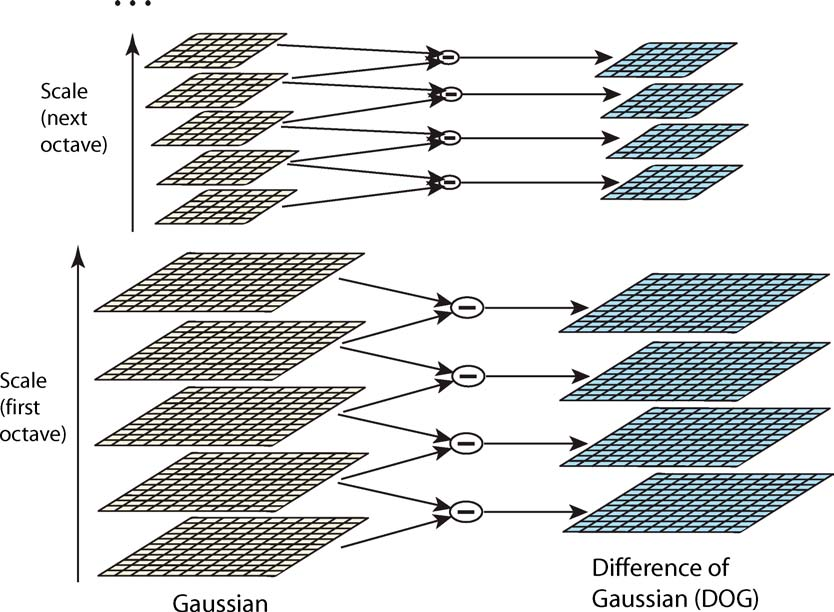
\includegraphics[width=0.8\textwidth]{Figures/sift/pyramid.jpg}
    \caption[DoG pyramid.]{DoG pyramid. \cite{Lowe2004}}
    \label{fig:DoG_pyramid}
\end{figure}

Each pixel in the DoG pyramid is compared to the $3\times3$ pixels in DoGs below and above, and to the $8$ surrounding pixels. This is shown in \figref{fig:DoG_extrema}. The pixel is selected as a key-point candidate, if it has lower or higher value than all of these $26$ pixels.

\begin{figure}
    \centering
    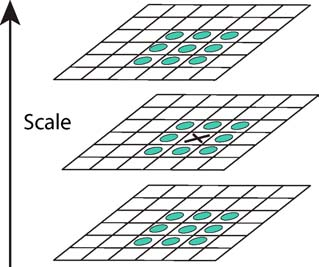
\includegraphics[width=0.4\textwidth]{Figures/sift/extrema.jpg}
    \caption[Optima of the DoG are selected by the means of comparing pixel to the 26 pixels surrounding it in the scale-space.]{Optima of the DoG are selected by the means of comparing pixel to the 26 pixels surrounding it in the scale-space. \cite{Lowe2004}}
    \label{fig:DoG_extrema}
\end{figure}

To detect a sub-pixel locations of extrema, the DoG is interpolated using quadratic Taylor expansion at each key-point candidate:
\begin{equation}
    D(\boldsymbol{x}) = D + \frac{\partial D^T}{\partial \boldsymbol{x}}\boldsymbol{x}+\frac{1}{2}\boldsymbol{x}^T\frac{\partial^2 D}{\partial \boldsymbol{x}^2}\boldsymbol{x},
    \label{eq:taylor_expansion}
\end{equation}
where \( D(x,y,\sigma) \) and the partial derivatives are evaluated at the key-point and \( \boldsymbol{x}=(x,y,\sigma) \) is the offset from the key-point. Then, extrema \( \hat{\boldsymbol{x}} \) is located by setting the gradient of \( D \) to be zero vector:
\begin{equation}
    \hat{\boldsymbol{x}} = - \frac{\partial^2 D^{-1}}{\partial \boldsymbol{x}^2}\frac{\partial D}{\partial \boldsymbol{x}}.
    \label{eq:taylor_extremum}
\end{equation}
If the offset \( \hat{\boldsymbol{x}} \) is larger than \( 0.5 \) in any dimension, it indicates that the extrema is closer to another point. In this case, the candidate point is changed to the new point and interpolation is performed again.

The function value at the sub-pixel extrema ,$D(\hat{\boldsymbol{x}})$, is used for rejecting extrema with low contrast. In our experiments, we use the OpenCV SIFT implementation default value $\frac{0.04}{3}$\cite{openCV}.

The DoG has a strong response along edges, even if the location along the edge is poorly determined. These candidate key-points have principal curvature perpendicular to the edge much larger than the principal curvature along it. The principal curvatures can be computed from a $2\times2$ Hessian matrix at the location of the key-point candidate
\begin{equation}
    \boldsymbol{H} =
    \begin{bmatrix}
        D_{xx} & D_{xy}\\
        D_{xy} & D_{yy}
    \end{bmatrix},
    \label{eq:hessian}
\end{equation}
where the partial derivatives are estimated by taking the differences of neighboring sample points. The eigenvalues of $\boldsymbol{H}$ are proportional to the principal curvatures.

The computation of eigenvalues can be avoided, as only the ratio of the eigenvalues is required. Let us denote the larger eigenvalue as $\alpha$ and the smaller one as $\beta$. The trace of $\boldsymbol{H}$ is defined as
\begin{equation}
    Tr(\boldsymbol{H}) = D_{xx}+D_{yy} = \alpha+\beta,
\end{equation}
and the determinant as
\begin{equation}
    Det(\boldsymbol{H}) = D_{xx}D_{yy}-D_{xy}^2 = \alpha\beta.
\end{equation}

Let $r$ be the ratio of the eigenvalues, such that
\begin{equation}
    r=\frac{\alpha}{\beta}.
\end{equation}
Then,
\begin{equation}
    \frac{Tr(H)^2}{Det(\boldsymbol{H})} = \frac{(\alpha+\beta)^2}{\alpha\beta}=\frac{(r\beta+\beta)^2}{r\beta^2} = \frac{(r+1)^2}{r}.
\end{equation}

Therefore, to inspect the ratio of eigenvalues, we can check
\begin{equation}
    \frac{Tr(H)^2}{Det(\boldsymbol{H})} = \frac{(\alpha+\beta)^2}{\alpha\beta}=\frac{(r\beta+\beta)^2}{r\beta^2} = \frac{(r+1)^2}{r}.
\end{equation}
The candidate key-points with this ratio below a threshold $r$ is discarded. In our experiments, we use the default value of OpenCV SIFT implementation: $10$.

\subsection{Key-point Description}
We want to create a descriptor for each of our key-points. These descriptors must be almost identical across different scale, rotation, illumination and other transformations.

In order to ensure descriptor invariance to a rotation, we first determine the key-point orientation. First, we calculate the gradient magnitude
\begin{equation}
    m(x,y) = \sqrt{(L(x+1,y)-L(x-1,y))^2+(L(x,y+1)-L(x,y-1))^2},
\end{equation}
and orientation
\begin{equation}
    \theta(x,y) = tan^{-1}\left(\frac{L(x,y+1)-L(x,y-1)}{L(x+1,y)-L(x-1,y)}\right),
\end{equation}
of each point within a region around the key-point. From these, an orientation histogram with $36$ bins is created. The largest peak is selected as a key-point orientation. If there are other peaks more than $80\%$ of the largest peak, new key-points are created at the same location with the other peaks as their orientation.

For the descriptor, a window $16\times16$ pixels around the key-point, rotated by the orientation of the key-point, is used. In this window, the gradient magnitude and the orientation is computed for each point. The $16\times16$ window is divided into $16$ ($4\times4$) sub-windows. For each sub-window, an $8$ bin gradient orientation histogram, weighted by gradient magnitudes, is created. This can be seen for smaller $8\times8$ window in \figref{fig:sift_descriptor}. These histograms then form a descriptor vector.

\begin{figure}
    \centering
    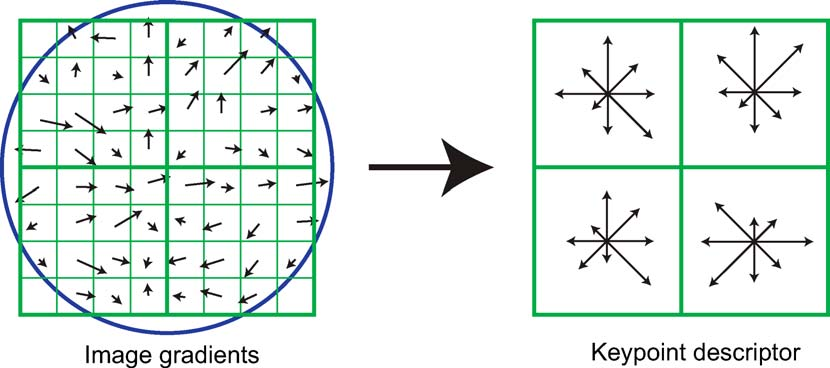
\includegraphics[width=0.8\textwidth]{Figures/sift/descriptor.jpg}
    \caption[Extracting the sift-descriptor.]{Building of the sift-descriptor. \cite{Lowe2004}}
    \label{fig:sift_descriptor}
\end{figure}


\section{Speeded Up Robust Features}
Speeded Up Robust Features (SURF) is a local feature transformation algorithm proposed by Herbert Bay, Tinne Tuytelaars, and Luc Van Gool in 2006 \cite{Bay2006}. Compared to SIFT \cite{Lowe1999}, the authors claim the SURF detector and descriptor to be faster and more robust against various image transformations.

\subsection{Key-point Detection}
The SURF key-point detection is based on the determinant of the Hessian matrix. Let us consider an input image $I_{img}(x,y)$ and the scale-space representation of the image
\begin{equation}
    L(x, y,\sigma) =  G(x,y,\sigma)*I_{img}(x,y),
\end{equation}
where $G(x,y,\sigma)$ is the Gaussian kernel defined in \eqref{eq:Gaussian_kernel}.

The Hessian matrix at scale $\sigma$ is defined as
\begin{equation}
    \mathcal{H}(x, y, \sigma) =
    \begin{bmatrix}
        L_{xx}(x, y, \sigma) & L_{xy}(x, y, \sigma)\\
        L_{xy}(x, y, \sigma) & L_{yy}(x, y, \sigma)
    \end{bmatrix},
\end{equation}
where $L_{xx}(x, y, \sigma)$, $L_{xy}(x, y, \sigma)$, and $L_{yy}(x, y, \sigma)$ are the second-order derivatives of the scale-space representation of the image at a point $(x, y)$.

The SURF authors decided to approximate the second order derivatives of Gaussian filter with box filters (shown in \figref{fig:Gauss_box_y}). Because the property of Gaussian filter, that no new structures can appear while going to a lower resolution, has been shown not to apply in 2D case \cite{Koenderink1984}, this can be done. Box filters allow for the use of integral images, which reduces the computational complexity.

\begin{figure}
    \centering
    \begin{subfigure}{0.24\textwidth}
        \centering
        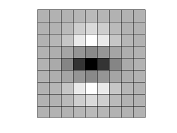
\includegraphics[width=\textwidth]{Figures/surf/y_gauss.png}
        \label{fig:y_gauss}
    \end{subfigure}
    \begin{subfigure}{0.24\textwidth}
        \centering
        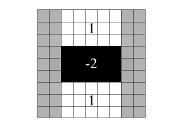
\includegraphics[width=\textwidth]{Figures/surf/y_box.png}
        \label{fig:y_box}
    \end{subfigure}
    \caption[Gaussian second-order derivative in the $y$-direction and its approximation using box filters]{Gaussian second order derivative in the $y$-direction and its approximation using box filters \cite{Bay2006}.}
    \label{fig:Gauss_box_y}
\end{figure}

Let us denote the approximations by $D_{xx}$, $D_{xy}$, and $D_{yy}$. The relative weights in the calculation of determinant of Hessian need to be weighted by $0.9$, which yields
\begin{equation}
    \text{det}(\mathcal{H}) = D_{xx} * D_{yy} - (0.9 * D_{xy})^{2}.
\end{equation}

Due to the use of box filters and integral images, any size of the box filter can be applied to the original image at the same speed directly. Therefore, the scale space is created by the use of up-scaled filters of sizes $9\times9$, $15\times15$, $21\times21$, $27\times27$, etc. For each octave, the difference between filter sizes is doubled (from $6$ to $12$ to $24$).

As the box filter layout remains the same, the corresponding Gaussian filter scales accordingly. The $9\times9$ box filter corresponds to a Gaussian filter with the scale $\sigma = 1.2$. Based on the definition of the process, we can calculate the corresponding Gaussian filter scale for each box filter size.

To select the key-points, non-maximum suppression in the $3\times3\times3$ neighborhood of each point is applied. Afterwards, the maxima of the determinant of the Hessian matrix are interpolated the same way as in the SIFT algorithm (using quadratic Taylor expansion).

\subsection{Key-point Description}
At first, we need to ensure the descriptor's invariance to rotation. For the key-point, we calculate the Haar-wavelet responses in the $x$ and the $y$ direction in a circular neighborhood of $6s$, where $s$ is the Gaussian filter scale at which the key-point was found. Integral images are used for speeding up the process.

The wavelet responses are weighted with a Gaussian($\sigma = 2.5 s$) centered at the key-point. The weighted responses are represented as vectors in a space with the $x$ response being a vector along the $x$-axis, and the $y$ response being a vector along the $y$-axis. All the vectors within a sliding window of $\frac{\pi}{3}$ are summed and the longest of the vector is selected as the key-point orientation.

An example of key-points and their orientation, found by OpenCV SURF implementation, can be seen in \figref{fig:surf_example}.
\begin{figure}[ht!]
    \centering
    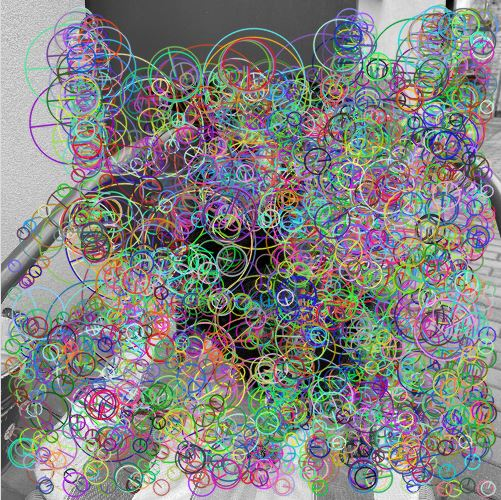
\includegraphics[width=0.50\textwidth]{Figures/surf/surf_example.jpg}
    \caption[SURF key-points and their orientation from an image of a dog]{SURF key-points and their orientation from an image of a dog.}
    \label{fig:surf_example}
\end{figure}

The descriptor is constructed from a square window the size of $20s$ around a key-point. The window is subsequently rotated along with the key-point orientation. Afterwards, this window is divided into $16$ ($4\times4$) square sub-windows. In each sub-window, the features are calculated using $5\times5$ regularly spaced sample points. From these sample points, we calculate the Haar wavelet responses in the horizontal and the vertical direction, where \say{horizontal} and \say{vertical} are defined in relation to the key-point orientation. The responses are weighted with a Gaussian ($\sigma = 3.3s$) centered at the key-point.

Let us call the horizontal responses $d_x$ and the vertical responses $d_y$. Over each sub-window, we denote the sum of the responses $\sum d_x$ and $\sum d_y$, and the sum of absolute values of the responses $\sum |d_x|$ and $\sum |d_y|$. The behavior of these values for different image patterns can be seen in \figref{fig:surf_descriptor}. Combining $\sum d_x$, $\sum d_y$, $\sum |d_x|$, and $\sum |d_y|$ for each of the $16$ sub-window into a vector, we get a descriptor of length $64$.

\begin{figure}
    \centering
    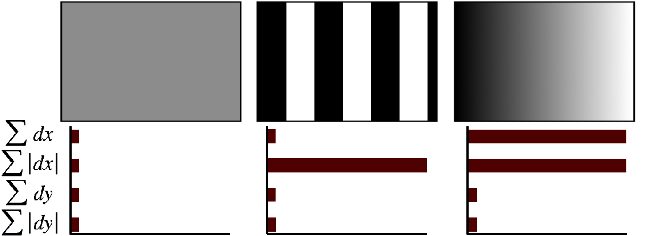
\includegraphics[width=0.8\textwidth]{Figures/surf/surf_descriptor.png}
    \caption[Behaviour of SURF descriptor for different image patterns]{Behaviour of SURF descriptor for different image patterns \cite{Bay2006}.}
    \label{fig:surf_descriptor}
\end{figure}


\section{ORB}
ORB (Oriented FAST and Rotated BRIEF) is a local feature extractor proposed by Ethan Rublee, Vincent Rabaud, Kurt Konolige and Gary Bradski in 2011 \cite{Rublee2011}.

The algorithm builds on a FAST (Features from Accelerated Segment Test) corner detector\cite{Rosten2006} and a BRIEF (Binary Robust Independent Elementary Features) descriptor\cite{Calonder2010}.

\subsection{Key-point Detection}
The ORB algorithm uses FAST-9 variant of the FAST corner detector. This detector compares each pixel intensity (denoted as $I_p$) in an image with the intensities of pixels in circle of radius $9$ around the pixel.

Let $n\in\mathbb{N}$ and threshold $t\in\mathbb{R}^{+}$ be given. Let $S$ be a set of pixels in a circle of radius $9$ around the examined pixel. Let us denote $I_x$ as the intensity of a pixel $x$. The examined pixel is selected as a corner, if there exists a set of $n$ contiguous pixels $S_n \in S$, where $\forall x \in S_n: I_x + t < I_p$, or $\forall x \in S_n: I_x - t > I_p$.

The selected corners, i.e. key-points are then ordered according to a Harris corner measure\cite{Harris1988}. For $N$ key-points, the threshold is selected low enough to get more than $N$ key-points, then the best $N$ key-points (according to Harris corner measure) are selected.

To find multi-scale features, the scale pyramid of an image is generated and key-points are generated at each level in the pyramid.

\subsection{Key-point Description}
To ensure the descriptor's invariance to rotation, we need to determine the key-point orientation. For this, the intensity centroid\cite{Rosin1999} is used. The intensity centroid expects the intensity of a key-point to be offset from its center. The vector from the center to the centroid is used for the key-point orientation.

Given an image $I(x,y)$, the centroid is found using a moment of a patch
\begin{equation}
    m_{pq}=\sum_{x,y} x^p y^q I(x,y).
\end{equation}
The centroid is then located as
\begin{equation}
    C =
    \begin{pmatrix}
        \frac{m_{10}}{m_{00}} \text{, } \frac{m_{01}}{m_{00}}
    \end{pmatrix},
\end{equation}
from which we can obtain the key-point orientation
\begin{equation}
    \theta = \text{atan}2(m_{01},m_{10}),
\end{equation}
where atan$2$ is the quadrant-aware version of arctan.

As an ORB descriptor, a variation on BRIEF descriptor is used. The BRIEF descriptor is a vector of binary values. This allows for fast matching using a Hamming distance.

The descriptor values is computed by comparing random pairs of pixel intensities in a patch. The binary vector is created from the responses on a patch $\boldsymbol{p}$ of test
\begin{equation}
    \tau(\boldsymbol{p};x,y)=
    \begin{cases*}
        1 & if $\boldsymbol{p}(x) < \boldsymbol{p}(y)$ \\
        0 & otherwise
    \end{cases*}, 
\end{equation}
where $\boldsymbol{p}(x)$ is the pixel intensity of a patch $\boldsymbol{p}$ at a point $x$, $x$ and $y$. The pairs of points $x$ and $y$ are from a random predetermined set
\begin{equation}
    \boldsymbol{S} =
    \begin{pmatrix}
        x_1 \dots x_n \\
        y_1 \dots y_n
    \end{pmatrix} 
\end{equation}
where $n$ is the size of our descriptor. The BRIEF descriptor is then defined as a vector of $n$ binary tests:
\begin{equation}
    f_n(\boldsymbol{p}) \coloneqq \sum_{i=1}^{n} 2^{i-1}\tau(\boldsymbol{p};x_i, y_i)
\end{equation}

The steered version of a BRIEF descriptor, according to the orientation $\theta$ of the key-point, can be created by using a corresponding rotation matrix $\boldsymbol{R}_\theta$:
\begin{equation}
    \boldsymbol{S_\theta} = \boldsymbol{R}_\theta \boldsymbol{S}.
\end{equation}
The sets of pairs are precomputed in a lookup table for discretized $\theta$ in increments of $\frac{2\pi}{30}$ to improve speed. In the end, the steered BRIEF descriptor becomes
\begin{equation}
    g_n(\boldsymbol{p}, \theta) \coloneqq f_n(\boldsymbol{p}) | (x_i, y_i) \in \boldsymbol{S}_\theta.
\end{equation}


\section{Bag of Visual Words}
Local feature extractors provide us with varied number of descriptors for each image. However, for classification, we require each image to be represented by a single vector. This can be achieved using a Bag of Words technique.

Bag of Words (BoW) is a technique, which represents each sample in a dataset as a multiset of its words. In general, these words do not have to be literal words but can be any categorization of information provided by the sample.

The first step of BoW is the dictionary generation. The dictionary is a set of $k \in \mathbb{N}$ categories of words called bins. Providing the dictionary, the BoW assigns each word to a bin. Finally, for each sample in the dataset, a histogram of frequencies of words belonging to each bin is calculated.

As an example, we explain the technique with text documents. With text documents, the dictionary consists of every unique word in all documents. The words of each document are assigned to a bin consisting of said words.

For example, in a dictionary consisting of bins [ \say{Peter}, \say{run}, \say{talked}, \say{to} ], a sample sentence \say{Peter talked to Peter} would produce the following histogram:
\begin{equation}
    [2, 0, 1, 1].
\end{equation}

In our case, we consider the descriptors found in an image as words. Since we are dealing with visual information, let us call these words \say{visual words} and designate the BoW technique \say{Bag of Visual Words} (BoVW).

We generate the categories using a $k$-means algorithm on all the visual words in the training dataset. Afterwards, we assign the visual words to the closest (considering euclidean distance) category and compute the histogram of frequencies.

\subsection{$k$-means}
The $k$-means algorithm is an unsupervised learning technique \cite{macqueen1967}. Let $X=\{ x_1, x_2, \dots, x_n \}$ be a dataset of $n$ data-points. The goal is to assign the data points into $k$ clusters $S = \{ S_1, S_2, \dots, S_k \}$, such that
\begin{equation}
    \argmin_S \sum_{i=1}^k \sum_{x\in S_i} \norm{x-c_i}^2,
\end{equation}
where \(c_1, c_2, ..., c_k \) are the centroids of corresponding clusters \(S_1, S_2, ..., S_k \). The centroids are determined as means of data points belonging to each cluster.

The algorithm starts by selecting $k$ random data points as the centroids. The iterative process is based on the alternation between the following two consecutive steps until a termination condition is met:
\begin{description}
    \item{\textbf{Assignment step:}} Each data point is assigned to the cluster, such that the Euclidean distance between the centroids of the clusters and the data point is the smallest one.
    \item{\textbf{Update step:}} For each cluster, a new centroid is computed as the mean value of data points belonging to this cluster.
\end{description}

The termination condition is satisfied, when the ratio of the samples, for which the assigned cluster changes, to the total amount of samples, is smaller than a specified threshold. The steps of the algorithm are demonstrated in \figref{fig:k_means_alg}.
\begin{figure}[ht]
    \centering
    \begin{subfigure}[t]{0.22\textwidth}
        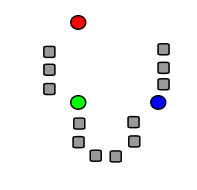
\includegraphics[width=\textwidth]{Figures/k-means/k-means_inicial_step.png}
        \caption{At first, random data points are selected as the initial $k$ centroids.}
        \label{fig:k-means-alg:inicial_step}
    \end{subfigure}\hfill
    \begin{subfigure}[t]{0.22\textwidth}
        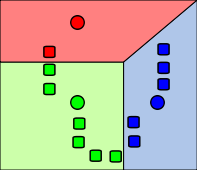
\includegraphics[width=\textwidth]{Figures/k-means/k-means_assignment_step.png}
        \caption{By choosing the nearest centroid, each data point is assigned to a corresponding cluster.}
        \label{fig:k-means-alg:assignment_step}
    \end{subfigure}\hfill
    \begin{subfigure}[t]{0.22\textwidth}
        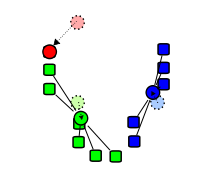
\includegraphics[width=\textwidth]{Figures/k-means/k-means_update_step.png}
        \caption{New centroids are calculated as mean values of data points in the cluster.}
        \label{fig:k-means-alg:update_step}
    \end{subfigure}\hfill
    \begin{subfigure}[t]{0.22\textwidth}
        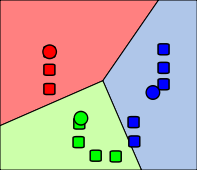
\includegraphics[width=\textwidth]{Figures/k-means/k-means_assignment_step_2.png}
        \caption{Steps in (b) and (c) are repeated until the terminate condition is met.}
        \label{fig:k-means-alg:assignment_step_2}
    \end{subfigure}\hfill
    \caption[Lloyd's algorithm demonstration.]{Lloyd algorithm demonstration \cite{Wikikmeans}.}
    \label{fig:k_means_alg}
\end{figure}
The challenge is the determination of the number of clusters $k$, the size of the visual dictionary. In our experiments, we examine different settings for $k$ to find a clustering, which allows for satisfactory classification.


\section{PCA}
PCA (Principal Component Analysis) is a global feature extractor. It is used to reduce the dimension of data while preserving as much of the data variance as possible.

Let $x_t \in \mathbb{R}^n$ be a data point, where $t=1,\dots,T$ and $T$ is the amount of data points. We want to project $x_t$ into a $y_t \in \mathbb{R}^k$, where $k < n$. We want to find the optimal parameters $P$ of the parametric reduction mapping $\psi_P: \mathbb{R}^n \rightarrow \mathbb{R}^k$ and the parametric reconstruction mapping $\psi_P^{-1}: \mathbb{R}^k \rightarrow \mathbb{R}^n$. The optimal parameters $P^{*}$ minimize the reconstruction error, i.e.,
\begin{equation}
    P^{*} \coloneqq \argmin_{P \in \rho} \sum_{t=1}^T \norm{x_t - \psi_P^{-1}(\psi_P(x_t))},
    \label{eq:mapping_optimization}
\end{equation}
where $\psi$ denotes the set of feasible parameters and $\norm{x_t - \psi_P^{-1}(\psi_P(x_t))}$ is the reconstruction error of a datapoint.

PCA uses the mappings
\begin{equation}
    \psi_{[Q,b]}^{-1}(y) \coloneqq Qy+b, \psi_{[Q,b]}(x) \coloneqq Q^{\top}(x-b),
    \label{eq:pca_mappings}
\end{equation}
with parameters $b \in \mathbb{R}^n$ and $Q \in \mathbb{R}^{n,k}$ with orthonormal columns, i.e.,
\begin{equation}
    Q^{\top}Q = I \in \mathbb{R}^{k,k}.
    \label{eq:pca_identity}
\end{equation}

Substituing \eqref{eq:pca_mappings}, \eqref{eq:pca_identity} into the optimization problem \eqref{eq:mapping_optimization} and using the square Euclidean norm for meassuring the reconstruction error, we get the optimization problem
\begin{equation}
    [Q^{*}, b^{*}] \coloneqq \argmin_{Q,b} \sum_{t=1}^T \norm{x_t - (QQ^{\top}(x_t-b) + b)}^2_2 \text{s.t.} Q^{\top}Q=I.
    \label{eq:pca_optimization}
\end{equation}
The objective function $f(Q,b)$ of \eqref{eq:pca_optimization} can be rewritten to the form
\begin{equation}
    f(Q,b)=\sum_{t=1}^T (x_t^{\top}x_t - 2 x_t^{\top}b + b^{\top}b - x_t^{\top}QQ^{\top}x_t + 2x_t^{\top}QQ^{\top}b - b^{\top}QQ^{\top}b),
    \label{eq:pca_obj_fun}
\end{equation}
and the optimality condition of $b^{*}$ can be formulated as
\begin{equation}
    \nabla_bf(Q,b) = \sum_{t=1}^T(-2x_t+2b+2QQ^{\top}xt-2QQ^{\top}b)=0,
\end{equation}
which is equivalent to
\begin{equation}
    (I-QQ^{\top})\sum_{t=1}^T(b-x_t)=0.
    \label{eq:pca_opt_b}
\end{equation}
As $k<n$, $Q \in \mathbb{R}^{n,k}$ is not a full column rank and $QQ^{\top} \neq = I$. The unique solution of \eqref{eq:pca_opt_b} is
\begin{equation}
    b^{*} = \frac{1}{T}\sum_{t=1}^T x_t.
\end{equation}
Moreover, the Hessian matrix
\begin{equation}
    \nabla_{b,b}^2 f(Q,b)=2(I-QQ^{\top}),
    \label{eq:pca_sol_b}
\end{equation}
is symmetric positive definitive matrix, therefore the objective function \eqref{eq:pca_obj_fun} is strictly convex (in the variable $b$) and \eqref{eq:pca_sol_b} is unique minimizer.

Let us denote the shifted data by
\begin{equation}
    \hat{x_t} \coloneqq x_t - b^* , t=1, \dots, T
\end{equation}
and write the objective function of \eqref{eq:pca_obj_fun} as
\begin{equation}
    f(Q,b^*) = \sum_{t=1}^T \norm{\hat{x_t} - QQ^{\top}\hat{x_t}}_2^2 = \sum_{t=1}^T (\hat{x_t}^{\top}\hat{x_t} - \hat{x_t}^{\top} QQ^{\top} \hat{x_t}).
    \label{eq:pca_obj_fun_Q}
\end{equation}
We can simplify \eqref{eq:pca_obj_fun_Q} using properties of the matrix trace:
\begin{equation}
    f(Q,b^*) = \sum_{t=1}^T \text{trace} (\hat{x_t}^{\top}\hat{x_t}) - \sum_{t=1}^T \text{trace} (\hat{x_t}^{\top} QQ^{\top} \hat{x_t})
    = \text{trace}(\text{cov}(x)) - \text{trace}(Q^{\top} \text{cov}(x) Q ),
\end{equation}
where cov($x$) is the covariance matrix of $x$ defined as
\begin{equation}
    \text{cov}(x) \coloneqq \sum_{t=1}^T(x_t-b^*)(x_t-b^*)^{\top} = \sum_{t=1}^T\hat{x_t}\hat{x_t}^{\top}.
\end{equation}
The argument of the minimum is independent of constants in the objective function. Therefore, we can reformulate the optimization problem \eqref{eq:pca_optimization} (in terms of variable $Q$) as
\begin{equation}
    \begin{split}
        [Q^*] &= \argmin_{Q^{\top}Q=I} f(Q,b^*) = \argmin_{Q^{\top}Q=I} -\text{trace}(Q^{\top}\text{cov}(x)Q) \\&= \argmax_{Q^{\top}Q=I} \text{trace}(Q^{\top}\text{cov}(x)Q) \\&= \argmax_{\forall j:q_j^{\top}q_j=1} \sum_{j=1}^k q_j^{\top} \text{cov}(x) q_j,
    \end{split}
    \label{eq:pca_optimization_final}
\end{equation}
where $q_j , j=1,\dots,k$ denote the (orthonormal) columns of the matrix $Q \in \mathbb{R}^{n,k}$. The Lagrange function corresponding to the problem \eqref{eq:pca_optimization_final} is given by
\begin{equation}
    L(Q, \lambda) \coloneqq \sum_{j=1}^k q_j^{\top} \text{cov}(x)q_j - \sum_{j=1}^k \lambda_j (q_j^{\top} q_j - 1),
\end{equation}
where $\lambda \in \mathbb{R}^K$ denotes Lagrange multiplier correponding to equality constraints. The first Karush-Kuhn-Tucker conditions can be derived as
\begin{equation}
    \nabla_{q_j}L(Q,\lambda) = 2 \text{cov}(x)q_j-2\lambda_jq_j=0, j=1,\dots,k,
\end{equation}
which are the eigenvalue equations
\begin{equation}
    \text{cov}(x)q_j=\lambda_j q_j, j=1,\dots,k.
    \label{eq:pca_eig}
\end{equation}
If we substitute \eqref{eq:pca_eig} into objective function \eqref{eq:pca_optimization_final}, we get
\begin{equation}
    \sum_{j=1}^k q_j^{\top} \text{cov}(x)q_j = \sum_{j=1}^k \lambda_j q_j^{\top}q_j = \sum_{j=1}^k \lambda_j.
\end{equation}
As the problem \eqref{eq:pca_optimization_final} is maximization problem, the optimal $Q^*$ consists of (orthonormal) eigenvectors which correspond to $k$ largest eigenvalues.




\chapter{Classifiers}
For data classification we are using two classification techniques, Bayes model and SVM. The goal of these techniques is to find a mapping from a feature space into a space of labels.

\section{Bayesian Model}
This classifier is suitable for classifying data, represented by a stochastic vector. The BoVW data can be easily transformed into such vector. Instead of each component of the BoVW vector representing the amount of key-points in respective category, the component in our new vector represents the probability of key-points belonging in respective category.

Let us denote the stochastic data vector $\Pi_{xt} \in \mathbb{R}^{K_x}, t=1,\dots,T$, where $T$ is the amount of samples. Let the vector $\Pi{yt}\in \mathbb{R}^{K_y}$ be vector of probabilities, with which $\Pi{xt}$ belongs to each category, and $K_y$ the amount of categories.

Given a stochastic data vector $\Pi_x$, we can describe the transformation $\mathbb{R}^{K_x} \rightarrow \mathbb{R}^{K_y}$ using a matrix $\Delta \in \mathbb{R}^{K_y, K_x}$:
\begin{equation}
    \Delta =
    \begin{bmatrix}
        P(\Pi_y^1 | \Pi_x^1) & P(\Pi_y^1 | \Pi_x^2) & \dots & P(\Pi_y^1 | \Pi_x^{K_x})\\
        P(\Pi_y^2 | \Pi_x^1) & P(\Pi_y^2 | \Pi_x^2) & \dots & P(\Pi_y^2 | \Pi_x^{K_x})\\
        \vdots & \ddots\\
        P(\Pi_y^{K_y} | \Pi_x^1) & P(\Pi_y^{K_y} | \Pi_x^2) & \dots & P(\Pi_y^{K_y} | \Pi_x^{K_x})
    \end{bmatrix},
\end{equation}
where $\Pi_x^n$ is the $n$-th element of $\Pi_x$, similar for $\Pi_y^n$, and the matrix $\Delta$ is a left stochastic matrix.

The search for the optimal $\Delta^{*}$ can be written as
\begin{equation}
    \Delta^* = \argmin_{\Delta \in \Omega_{\Delta}} \sum_{t=1}^T \text{dist}(\Pi_{yt}, \Delta\Pi_{xt}),
\end{equation}
where $\Omega_{\Delta}$ is a set of left stochastic matrices. The dist($\Pi_{yt}, \Delta\Pi_{xt}$) is calculated as Kullback-Leiber divergence\cite{Kullback1951}:
\begin{equation}
    \text{dist}(\Pi_{yt}, \Delta\Pi_{xt}) = - \sum_{i=1}^{K_y} \Pi_{yt}^i \ln\frac{(\Delta\Pi_{xt})_i}{\Pi_{yt}^i} = - \sum_{i=1}^{K_y} \Pi_{yt}^i (\ln (\Delta\Pi_{xt})_i - \ln \Pi_{yt}^i).
\end{equation}
For the purpose of optimization, the term $\ln \Pi_{yt}^i$ is constant, therefore it can be ignored:
\begin{equation}
    \text{dist}(\Pi_{yt}, \Delta\Pi_{xt}) \propto - \sum_{i=1}^{K_y} \Pi_{yt}^i \ln (\Delta\Pi_{xt})_i.
\end{equation}
This problem is hard to minimize analytically. However, $\Delta\Pi_{xt}$ is a convex function, and therefore $-\ln(\Delta\Pi_{xt})$ is a convex function. Thus Jensen's inequality can be used:
\begin{equation}
    - \sum_{i=1}^{K_y} \Pi_{yt}^i \ln (\Delta\Pi_{xt})_i \leq - \sum_{i=1}^{K_y} \Pi_{yt}^i ( \sum_{j=1}^{K_x} \Pi_{xt}^j \ln (\Delta_{ij}) ) = - \sum_{i=1}^{K_y} \sum_{j=1}^{K_x} \Pi_{yt}^i \Pi_{xt}^j \ln \Delta_{ij}.
\end{equation}
From this, we get an optimization problem
\begin{equation}
    \Delta^* = \argmin_{\Delta \in \Omega_{\Delta}} - \sum_{t=1}^T \sum_{i=1}^{K_y} \sum_{j=1}^{K_x} \Pi_{yt}^i \Pi_{xt}^j \ln \Delta_{ij},
\end{equation}
where
\begin{equation}
    \Omega_{Delta} = \{ \Delta \in [0, 1], \forall j \in \{ 1, 2, \dots, K_x \} : \sum_{i=1}^{K_y} \Delta_{ij} = 1 \},
\end{equation}
which can be solved analytically.

Let $\Delta$ be the optimal stochastic matrix. There exist $\lambda_j \in \mathbb{R}^{K_x}$ such that
\begin{equation}
    L(\Delta, \lambda) = - \sum_{t=1}^T \sum_{i=1}^{K_y} \sum_{j=1}^{K_x} \Pi_{yt}^i \Pi_{xt}^j \ln \Delta_{ij} + \sum_{j=1}^{K_x} \lambda_j (\sum_{i=1}^{K_y} \Delta_{ij} - 1)
\end{equation}
is the Lagrange function. We can find the optimal $\Delta^*$:
\begin{equation}
    \nabla_{\Delta_{\hat{i}\hat{j}}} L(\Delta_{\hat{i}\hat{j}}, \lambda) = - \frac{1}{\Delta_{\hat{i}\hat{j}}} \sum_{t=1}^{T} \Pi_{yt}^{\hat{i}} \Pi_{xt}^{\hat{j}} + \lambda_{\hat{j}} = 0,
\end{equation}
\begin{equation}
    \nabla_{\Delta_{\hat{j}}} = \sum_{i=1}^{K_y} \Delta_{i\hat{j}} - 1 = 0,
\end{equation}
\begin{equation}
    \Delta_{\hat{i}\hat{j}} = \frac{\sum_{t=1}^{T} \Pi_{yt}^{\hat{i}} \Pi_{xt}^{\hat{j}}}{\lambda{\hat{j}}},
\end{equation}
\begin{equation}
    \lambda_{\hat{j}} = \sum_{i=1}^{K_y} \sum_{t=1}^{T} \Pi_{yt}^{i} \Pi_{xt}^{\hat{j}},
\end{equation}
\begin{equation}
    \Delta_{\hat{i}\hat{j}}^{*} = \frac{\sum_{t=1}^{T} \Pi_{yt}^{\hat{i}} \Pi_{xt}^{\hat{j}}}{\sum_{i=1}^{K_y} \sum_{t=1}^{T} \Pi_{yt}^{i} \Pi_{xt}^{\hat{j}},}.
\end{equation}

Another approach to finding the optimal $\Delta^{*}$, is optimizing the problem
\begin{equation}
    \Delta^* = \argmin_{\Delta \in \Omega_{\Delta}} - \sum_{t=1}^T \sum_{i=1}^{K_y} \Pi_{yt}^i \ln (\Delta\Pi_{xt})_i,
\end{equation}
without using the Jensen inequality.
As $-\ln(\Delta\Pi_{xt})$ is a convex function, the problem can be solved numerically using Spectral Projected Gradient method\cite{birgin2000}.

We use both approaches (the analytical solution using Jensen inequality and the numerical solution) in our experiments.


\section{SVM}
The SVM (Support Vector Machine) is a supervised learning classifier originally designed for binary classifications. It was introduced by Vladimir N. Vapnik and Alexey Ya. Chervonenkis in 1963 \cite{Cortes1995}.

Let \( T := \{(\boldsymbol{x_1}, y_1),(\boldsymbol{x_2}, y_2),...,(\boldsymbol{x_n}, y_n)\} \),
be the training dataset, where $n$ is the number of the samples, \( \boldsymbol{x_i} \in \mathbb{R}^m \), \( i \in \{1,2,\dots,n\} \),
is the sample and \( y_i \in \{-1, 1\} \) is the label related to the sample \( \boldsymbol{x_i} \). The classification model is represented by the means of the hyperplane \( H \), defined such that:
\begin{equation}
    H: \boldsymbol{\omega}^T\boldsymbol{x}-\widetilde{b}=0,
    \label{eq:svm:hyperplane}
\end{equation}
where \( \omega \) is the normalized normal vector of the hyperplane \( H \), and
\begin{equation}
    \widetilde{b} = \frac{b}{\norm{\omega}}
    \label{eq:svm:offset}
\end{equation}
is the bias from the origin.

First, we consider linearly separable training data. The two classes of data are distinguished by two hyperplanes so that the distance between them is maximized. The region bound by these hyperplanes is called the margin. The hyperplane that lies halfway between them is called the maximum-margin hyperplane. These hyperplanes are described by the followin equation:
\begin{equation}
    \boldsymbol{w}^T\boldsymbol{x}-\widetilde{b}=\pm1.
    \label{eq:svm_hyperplanes}
\end{equation}
The sample $x_i, i=1,\dots,n$ belongs to the positive class, i.e. $y_i = 1, i=1,\dots,n$, when
\begin{equation}
    \boldsymbol{w}^T\boldsymbol{x_i}-\widetilde{b}\geq1
    \label{eq:svm_positive_data}
\end{equation}
and the negative class, i.e. $y_i = -1, i=1,\dots,n$
\begin{equation}
    \boldsymbol{w}^T\boldsymbol{x_i}-\widetilde{b}\leq-1.
    \label{eq:svm_negative_data}
\end{equation}
The properties \eqref{eq:svm_positive_data} and \eqref{eq:svm_negative_data} can be combined into a single equation
\begin{equation}
    y_i(\boldsymbol{w}^T\boldsymbol{x}-\widetilde{b})\geq1.
\end{equation}

\begin{figure}[ht!]
    \centering
    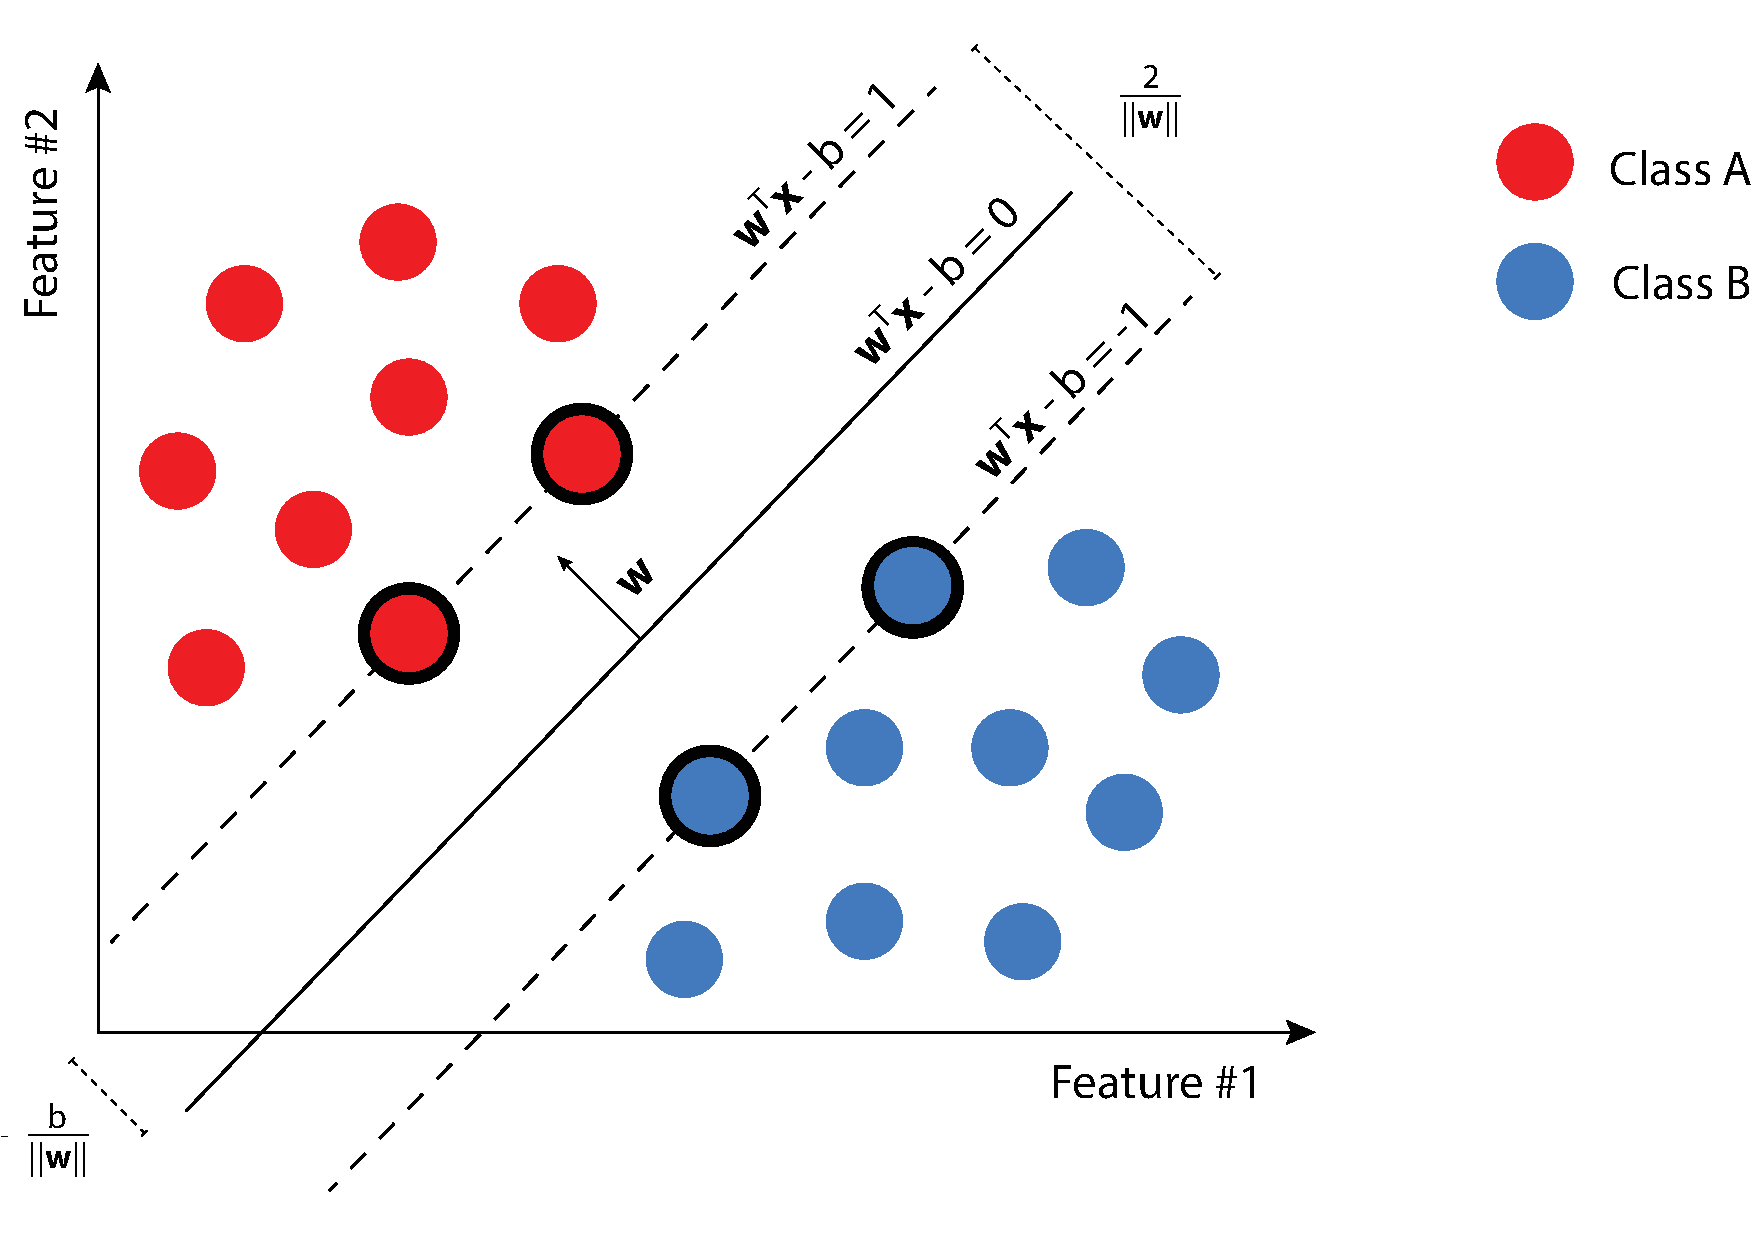
\includegraphics[width=0.6\textwidth]{Figures/svm/hyperplane_svm.pdf}
    \caption[Example of the SVM model.]{Example of the SVM model. \cite{Kruzik2018}}
    \label{fig:svm-margin}
\end{figure}

From the \figref{fig:svm-margin}, we can see, the distance between hyperplanes \eqref{eq:svm_hyperplanes} is \( \frac{2}{\norm{\boldsymbol{w}}} \). As we want to maximize this distance, we need to minimize $\norm{\boldsymbol{w}}$. This leads to an optimization problem
\begin{equation}
    \argmin_{\boldsymbol{w},b} \|\boldsymbol{w}\| \text{ s.t. }
    \begin{cases}
        y_i(\boldsymbol{w}^T\boldsymbol{x}_i-b)\geq1,\\
        i=1, ...,n,
    \end{cases}
\end{equation}
which can be reformulated as the Quadratic Programming problem
\begin{equation}
    \argmin_{\boldsymbol{w},b} \frac{1}{2}\|\boldsymbol{w}\|^2 \text{ s.t. }
    \begin{cases}
        y_i(\boldsymbol{w}^T\boldsymbol{x}_i-b)\geq1,\\
        i=1, ...,n.
    \end{cases}
    \label{eq:svm_hard_margin_minimization}
\end{equation}

Because the training data is nearly never linearly separable, the soft margin version of the SVM was proposed by Vladimir N. Vapnik and Corinna Cortes \cite{Cortes1995} in 1995. It exploits an additional function called the hinge loss function:
\begin{equation}
    \xi_i = \max(0, 1-y_i(\boldsymbol{w}^T\boldsymbol{x}_i-b)).
    \label{eq:svm_hinge_loss}
\end{equation}

The hinge loss function \eqref{eq:svm_hinge_loss} equals $0$ for a sample on the correct side of the corresponding hyperplane \eqref{eq:svm_hyperplanes}. However, for a sample on the wrong side of the corresponding hyperplane \eqref{eq:svm_hyperplanes}, the value of the function is proportional to the distance from the hyperplane.

If we add the hinge loss function \eqref{eq:svm_hinge_loss} to the optimization problem \eqref{eq:svm_hard_margin_minimization}, we get a soft margin SVM optimization problem
\begin{equation}
    \argmin_{\boldsymbol{w},b,\xi_i} \frac{1}{2}\|\boldsymbol{w}\|^2 + C\sum_{i = 1}^n\xi_i \text{ s.t. }
    \begin{cases}
        y_i(\boldsymbol{w}^T\boldsymbol{x}_i-b)\geq1 - \xi_i,\\
        \xi_i \geq 0 , i=1, ...,n.
    \end{cases}
    \label{eq:svm:soft_margin_minimization}
\end{equation}
where \( C \) is a penalty for the misclassification error. The formulation \eqref{eq:svm:soft_margin_minimization} is called the $l1$-loss $l2$-regularized SVM. The primal formulation \eqref{eq:svm:soft_margin_minimization} can be modified using the Lagrange duality with Lagrange multipliers $\boldsymbol{\alpha} = [\alpha_1, \alpha_2, ..., \alpha_n]^{\top}$, $\boldsymbol{\beta} = [\beta_1, \beta_2, ..., \beta_n]^{\top}$. Exploiting Karush-Kuhn-Tucker conditions, we obtain the dual formulation
\begin{equation}
    \argmin_{\boldsymbol{\alpha}} \frac{1}{2} \boldsymbol{\alpha}^T\boldsymbol{Y}^T\boldsymbol{K}\boldsymbol{Y}\boldsymbol{\alpha} - \boldsymbol{\alpha}^T\boldsymbol{e} \text{ s.t. } 
    \begin{cases}
        \boldsymbol{o} \leq \boldsymbol{\alpha} \leq C\boldsymbol{e},\\
        \boldsymbol{B_e}\boldsymbol{\alpha}=0,
    \end{cases}
    \label{eq:svm:soft_margin_dual}
\end{equation}
where \( \boldsymbol{e} = [1,1, ...,1]^{\top} \), \( \boldsymbol{o} = [0,0, ...,0]^{\top} \), \( \boldsymbol{X} = [\boldsymbol{x_1},\boldsymbol{x_2}, ...,\boldsymbol{x_n}] \), \( \boldsymbol{y} = [y_1,y_2, ...,y_n]^{\top} \), \( Y = \text{diag}(\boldsymbol{y}) \), \( \boldsymbol{B_e} = [\boldsymbol{y}^T] \) and \( \boldsymbol{K}\coloneqq\boldsymbol{X}^T\boldsymbol{X} \) is the Gram matrix which is symetric positive semi-definite (SPSD)\cite{Aeta2018}. The Hessian matrix in \eqref{eq:svm:soft_margin_dual}
\begin{equation}
    \boldsymbol{H} \coloneqq \boldsymbol{Y}^T\boldsymbol{X}^T\boldsymbol{X}\boldsymbol{Y}
    \label{eq:svm:hessian}
\end{equation}
is also SPSD matrix.

To recover the normal vector, the formula
\begin{equation}
    \boldsymbol{w}=\boldsymbol{X}\boldsymbol{Y}\boldsymbol{\alpha}.
    \label{eq:svm:dual_to_primal_w}
\end{equation}
is used. The bias $b$ can be recovered as
\begin{equation}
    b=\boldsymbol{w}\cdot \boldsymbol{\Bar{x}} - y_i,
    \label{eq:svm:dual_to_primal_b}
\end{equation}
where $\boldsymbol{\Bar{x}}$ is the mean of all support vectors.

Instead of the linear sum of the loss functions $\xi_i$ in \eqref{eq:svm:soft_margin_minimization}, we can use the square sum of the loss functions in the objective function
\begin{equation}
    \argmin_{\boldsymbol{w},b,\xi_i} \frac{1}{2}\|\boldsymbol{w}\|^2 + \frac{C}{2}\sum_{i = 1}^n\xi_i^2 \text{ s.t. } 
    \begin{cases}
        y_i(\boldsymbol{w}^T\boldsymbol{x}_i-b)\geq1 - \xi_i,\\
        i=1, ...,n.
    \end{cases}
    \label{eq:svm:soft_margin_minimization_l2}
\end{equation}
The problem \eqref{eq:svm:soft_margin_minimization_l2} is called $l2$-loss $l2$-regularized SVM. The dual formulation can again be optained by using the Lagrange duality:
\begin{equation}
    \argmin_{\boldsymbol{\alpha}} \frac{1}{2} \boldsymbol{\alpha}^T(\boldsymbol{H}+C^{-1}\boldsymbol{I})\boldsymbol{\alpha} - \boldsymbol{\alpha}^Te \text{ s.t. } 
    \begin{cases}
        \boldsymbol{o} \leq \boldsymbol{\alpha},\\
        \boldsymbol{B_e}\boldsymbol{\alpha}=0.
    \end{cases}
    \label{eq:svm:soft_margin_dual-l2}
\end{equation}

The Hessian matrix $\boldsymbol{H}$, regularized by the matrix $C^{-1}\boldsymbol{I}$ is symmetric positive definite, therefore, this optimization problem should be more stable than the $l1$-loss $l2$-regularized SVM problem.


\section{Metrics}
To assess the quality of the classification model, we need to analyze several metrics. Many of such metrics are derived from a confusion matrix (see \tabref{tab:confusion_matrix}).
\begin{table}[ht]
    \centering
    \begin{tabular}{|c|c|c|}
        \hline
        & Predicted negative & Predicted positive \\ 
        \hline 
        Actual negative & True negatives ($TN$) & False positives ($FP$) \\ 
        \hline
        Actual positive & False negatives ($FN$) & True positives ($TP$)  \\ 
        \hline
    \end{tabular}
    \caption{Confusion Matrix}
    \label{tab:confusion_matrix}
\end{table}
The confusion matrix is generated by counting the testing data, which are supposed to belong to a negative class (Actual negative) or a positive class (Actual positive), and their predicted class (Predicted negative/Predicted positive).

We are considering the following metrics in our experiments:
\begin{description}
    \item{\textbf{Accuracy:}} How often is the classifier correct overall. This metric is represented in percentages.
    \begin{equation}
        \frac{TN+TP}{TN+FP+FN+TP}
        \label{eq:svm:accuracy}
    \end{equation}
    \item{\textbf{Precision:}} How often is the classifier correct when it predicts positive.
    \begin{equation}
        \frac{TP}{TP+FP}
        \label{eq:svm:precision}
    \end{equation}
    \item{\textbf{Sensitivity (Recall):}} How often is the classifier correct when it is actually positive.
    \begin{equation}
        \frac{TP}{TP+FN}
        \label{eq:svm:sensitivity}
    \end{equation}
    \item{\textbf{\( F_1 \) Score:}} A harmonic mean of precision and sensitivity.
    \begin{equation}
        2\times\frac{\text{precision}\times\text{recall}}{\text{precision}+\text{recall}}
        \label{eq:svm:F1}
    \end{equation}
\end{description}

Generally, for each of these metrics, the higher value we get, the better the classification model.



\chapter{Datasets}
To test our extraction-classification pipeline, we use three progressively more complex datasets. We start by classifying simple 2D shapes, then move on to simple 3D shapes, and last, we attempt to classify a dataset of real photographs of cats and dogs.

Each dataset is split into a training and a testing subset. This ensures that we can test, how the classifier performs on unseen data.

\section{2D Shapes Dataset}
For the simplest dataset, we use a four shapes dataset \cite{kaggleFourShapes}. The dataset contains $16$,$000$ images of four shapes: square, star, circle, and triangle. The dataset was created from poster board cutouts of each shape painted green. While rotating, each shape was recorded using a Garmin Virb 1080p action camera for two minutes. Shapes were then cropped out from the frames of the video and resized to $200\times200$ pixels. The green color of the cutouts in frames was then changed to a pure black color, while the rest of the image was changed to a pure white color. An example of the data can be seen in \figref{fig:four_shapes}.
\begin{figure}[ht!]
    \centering
    \begin{subfigure}[t]{0.2\textwidth}
        
\includegraphics[width=\textwidth]{Figures/datasets/circle.png}
        \caption{Circle}
    \end{subfigure}
    \begin{subfigure}[t]{0.2\textwidth}
        
\includegraphics[width=\textwidth]{Figures/datasets/star.png}
        \caption{Star}
    \end{subfigure}
    \caption[Photographs of a circle and a star from the Four Shapes dataset]{Photographs of a circle and a star from the Four Shapes dataset \cite{kaggleFourShapes}.}
    \label{fig:four_shapes}
\end{figure}

As we are doing binary classification, we use only the pair of a circle (positive class) and a star (negative class). We assign $\sfrac{2}{3}$ of random images from each class to a training subset, and $\sfrac{1}{3}$ to a testing subset.

\section{3D Shapes Dataset}
The 3D Shapes dataset contains $20$ images of a box (positive class) and $20$ images of a sphere (negative class) viewed from differnt angles. The shapes are colored red, while the background is colored white. The objects are illuminated by a single light source, providing a nice and sharp shadow and shading of each shape. The dataset was generated by Ing. Lukáš Pospíšil, Ph.D. using POV-Ray software \cite{povray}. Each of the images is $300\times200$ pixels. An example of each shape can be seen in \figref{fig:3d_shapes}.
\begin{figure}[ht]
    \centering
    \begin{subfigure}[t]{0.2\textwidth}
        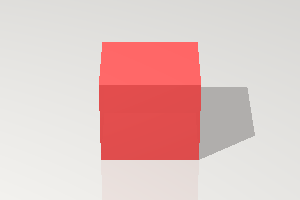
\includegraphics[width=\textwidth]{Figures/datasets/box.png}
        \caption{Box}
    \end{subfigure}
    \begin{subfigure}[t]{0.2\textwidth}
        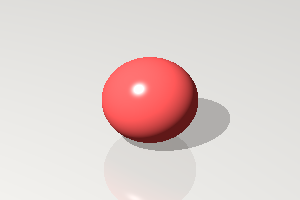
\includegraphics[width=\textwidth]{Figures/datasets/sphere.png}
        \caption{Sphere}
    \end{subfigure}
    \caption[3D shapes, generated by Ing. Lukáš Pospíšil, Ph.D. in POV-Ray]{3D shapes, generated by Ing. Lukáš Pospíšil, Ph.D. in POV-Ray \cite{povray}.}
    \label{fig:3d_shapes}
\end{figure}

We assign $\sfrac{2}{3}$ of random images from each class to a training subset, and $\sfrac{1}{3}$ to a testing subset.

\section{Cats and Dogs Dataset}\label{sec:cat_dog_dataset}
The Cats and Dogs dataset is created from the Oxford-IIIT Pet Dataset \cite{parkhi12a}. As the original dataset contains a few damaged images, we use a fixed version of the dataset from \cite{ml4py_dataset}.

The dataset contains over $7$,$000$ images of different cat and dog breeds, example of a cat and a dog image can be seen in \figref{fig:iiit_pet}.
\begin{figure}[!htp]
    \centering
    \begin{subfigure}[t]{0.45\textwidth}
        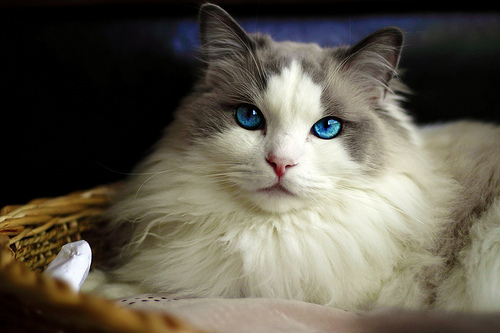
\includegraphics[width=\textwidth]{Figures/datasets/cat.jpg}
        \label{fig:original:example_cat}
    \end{subfigure}\hfill
    \begin{subfigure}[t]{0.45\textwidth}
        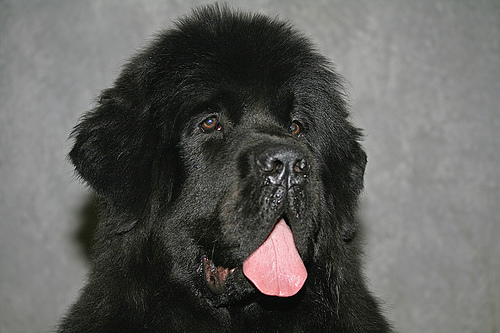
\includegraphics[width=\textwidth]{Figures/datasets/dog.jpg}
        \label{fig:original:example_dog}
    \end{subfigure}
    \caption[Example of images depicting a cat (left) and a dog (right) in the Oxford-IIIT Pet Dataset]{Example of images depicting a cat (left) and a dog (right) in the Oxford-IIIT Pet Dataset \cite{parkhi12a}.}
    \label{fig:iiit_pet}
\end{figure}
The classes in the dataset are unbalanced, there are approximately twice as many images of dogs as there are of cats.

The dataset provides us with a trimap for each image. The trimap provides us with the information, which of the pixels are of the animal and which are of the background. We use these to cut out the animal from the background (set all the background pixel values to black). An example of this can be seen in \figref{fig:iiit_pet_cutout}.
\begin{figure}[!htp]
    \centering
    \begin{subfigure}{0.5\textwidth}
        \begin{subfigure}[t]{0.45\textwidth}
            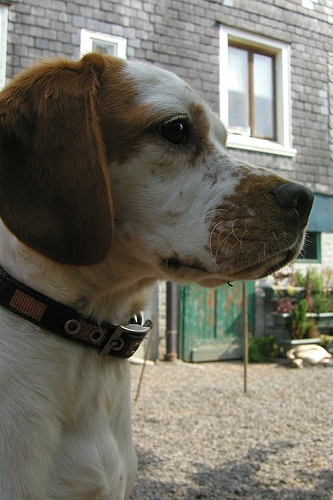
\includegraphics[width=\textwidth]{Figures/datasets/beagele.jpg}
            \label{fig:original:example}
        \end{subfigure}\hfill
        \begin{subfigure}[t]{0.45\textwidth}
            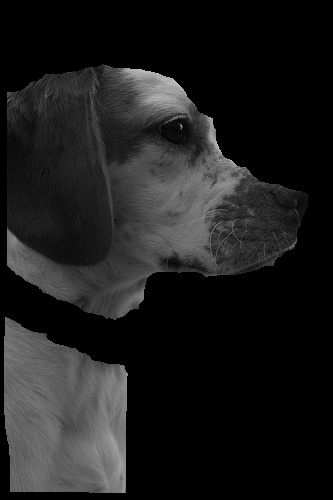
\includegraphics[width=\textwidth]{Figures/datasets/beagle_nobkg.jpg}
            \label{fig:pet:example}
        \end{subfigure}
    \end{subfigure}
    \caption[Original of a photograph of a beagle (left) and a cutout (right).]{Original of a photograph of a beagle (left) and a cutout (right) \cite{parkhi12a}.}
    \label{fig:iiit_pet_cutout}
\end{figure}

We assign the positive class to images of cats, and the negative class to images of dogs. In the original dataset,` we are provided with a training and testing subset. However, the ratio of training and testing samples in these classes is approximately $1:1$. To get a better representation of the data, we split the dataset ourselves, where we assign $90\%$ of the data to a training subset and $10\%$ of the data to a testing subset. The data is selected at random, making sure that for each breed of a cat or a dog, the ratio of amounts of training samples to testing samples is kept the same.


\chapter{Results}
In this chapter, we take a look at results of our classification. The whole pipeline is run on the Salomon supercomputer at IT4Innovations \cite{Salomon-WWW-17}. Each task was computed on a single compute node. Each compute node contains two 2.5 GHz, 12-core Intel Xeon E5-2680v3 (Haswell) processors and 128 GB of memory.

\section{Tools}
The data preprocessing and feature extraction of the Cats and Dogs dataset are done using the tools-iiit-pet from our ml4py toolkit \cite{tools_iiit}. The tool for the data preparation and feature extraction of the other two datasets is strongly inspired by the tools-iiit-pet tool.

For the local features extraction, we use the implementation of SIFT, SURF, and ORB from the OpenCV library \cite{opencv} and $k$-means implementation from the SciPy library \cite{scipy}. The BoVW is created in Python.

The global feature extractor, PCA, is implemented using PETSc \cite{petsc} and SLEPc \cite{slepc} libraries.

The Bayesian Model classifier using the Jensen inequality is implemented in python. The Bayesian Model solved using the Spectral Projected Gradient method is trained using an Octave code provided by Ing. Lukáš Pospíšil, Ph.D., while the testing is done in python.

For the SVM classification, we use the PermonSVM \cite{permonSVM}. This implementation of the SVM algorithm comes from the Department of Applied Mathematics, VSB-TUO, and the Institute of Geonics of the Czech Academy of Science in Ostrava, Czech Republic. It is build on top of a package for large scale quadratic programming, PermonQP. Both, PermonSVM and PermonQP, make use of the PETSc \cite{petsc} library.

\section{2D Shapes Dataset Classification}
In the 2D Shapes classification, we attempt to train and classify images of a circle, labeled as the positive data, and images of a star, labeled as the negative data. See section \ref{sec:2d-dataset} for details of benchmark formulation.

For local extractors, we examine the classification of BoVW with dictionary sizes $2, 3, 4, 6, 8, 12, 16$.

\subsection{SVM}

\begin{table}[ht!]
    \centering
    \input tables/pca_head

\rowcolor{LightCyan}
12&0.72&0.63&0.44&0.44&0.61&0.61&7.66&794.15&0.44&5.30&0.01&10001&16\\
\hline

\end{tabular}

    \caption[2D Shapes result for PCA extraction and SVM classification]{2D Shapes result for PCA extraction and SVM classification. \say{Ext} is shorthand for \say{Extraction}.}
    \label{tab:2d_PCA_SVM}
\end{table}
In \tabref{tab:2d_PCA_SVM}, we present results of the classification by the SVM model on data extracted using PCA. We keep only the first $n$ eigenvectors, which can together explain at least $95\%$ of the data variance. For the 2D Shapes dataset, we keep the first $12$ eigenvectors.

Both, the $l_1$ and the $l_2$ SVM, classified the testing data quite well as we can see from the score. However, by the number of itterations, we can see that the $l_1$-loss SVM model was unable to converge in less than $10,000$ itterations, and therefore it was stopped early.

\begin{table}[ht!]
    \centering
    \begin{tabular}{|c|c|c|c|c|c|c|c|c|c|c|c|}

\hline
\multirow{3}{*}{\shortstack[c]{Size\\of\\BoVW}}&\multicolumn{6}{c|}{Classification score}&\multicolumn{5}{c|}{Elapsed time [s]}\\
\cline{2-12}
&\multicolumn{2}{c|}{Accuracy}&\multicolumn{2}{c|}{Precission}&\multicolumn{2}{c|}{$F_1$}&\multirow{2}{*}{\shortstack[c]{Extraction}}&\multicolumn{2}{c|}{HyperOpt}&\multicolumn{2}{c|}{Training}\\
\cline{2-7}\cline{9-12}
&$l_1$&$l_2$&$l_1$&$l_2$&$l_1$&$l_2$&&$l_1$&$l_2$&$l_1$&$l_2$\\
\hline

\hline
\rowcolor{LightCyan}
2&0.97&0.86&0.96&0.90&0.97&0.87&33.81&28.50&21.94&1.88&0.17\\
\hline
3&0.99&0.92&1.00&0.96&0.99&0.92&33.93&34.21&38.23&0.36&0.15\\
\hline
\rowcolor{LightCyan}
4&0.92&1.00&0.85&1.00&0.92&1.00&32.67&11.72&8.37&0.24&0.13\\
\hline
6&1.00&1.00&1.00&1.00&1.00&1.00&32.92&4.27&3.78&0.09&0.07\\
\hline
\rowcolor{LightCyan}
8&1.00&1.00&1.00&1.00&1.00&1.00&34.60&4.98&5.07&0.13&0.07\\
\hline
12&1.00&1.00&1.00&1.00&1.00&1.00&36.15&4.14&3.45&0.08&0.07\\
\hline
\rowcolor{LightCyan}
16&1.00&1.00&1.00&1.00&1.00&1.00&36.53&4.61&3.87&0.08&0.07\\
\hline
\end{tabular}

    \caption[2D Shapes results for extraction: SIFT and classification: SVM]{2D Shapes results for extraction: SIFT and classification: SVM.}
    \label{tab:2d_SIFT_SVM}
\end{table}
In \tabref{tab:2d_SIFT_SVM}, we can see results of the classification by the SVM model on data extracted using SIFT. Since the data is quite simple, the classifier has no problem classifying the data for any size of the BoVW dictionary. However, we can see, that both, the SVM-l1 and SVM-l2, converged much faster for larger sizes of the BoVW dictionary. Moreover, we recieved perfect score for accuracy, precission, and $F_1$ from the BoVW sizes beyond the size of $6$.

\begin{table}[ht!]
    \centering
    \begin{tabular}{|c|c|c|c|c|c|c|c|c|c|c|c|}

\hline
\multirow{3}{*}{\shortstack[c]{Size\\of\\BoVW}}&\multicolumn{6}{c|}{Classification score}&\multicolumn{5}{c|}{Elapsed time [s]}\\
\cline{2-12}
&\multicolumn{2}{c|}{Accuracy}&\multicolumn{2}{c|}{Precission}&\multicolumn{2}{c|}{$F_1$}&\multirow{2}{*}{\shortstack[c]{Extraction}}&\multicolumn{2}{c|}{HyperOpt}&\multicolumn{2}{c|}{Training}\\
\cline{2-7}\cline{9-12}
&$l_1$&$l_2$&$l_1$&$l_2$&$l_1$&$l_2$&&$l_1$&$l_2$&$l_1$&$l_2$\\
\hline

\hline
\rowcolor{LightCyan}
2&0.96&0.96&0.92&0.91&0.96&0.95&10.4&6.0&10.2&0.2&0.2&385&353\\
\hline
3&0.74&0.72&0.48&0.44&0.65&0.61&10.3&10.3&11.5&0.3&0.3&645&500\\
\hline
\rowcolor{LightCyan}
4&0.97&0.98&1.00&1.00&0.98&0.98&10.3&19.2&19.4&0.3&0.3&614&643\\
\hline
6&0.98&0.98&1.00&1.00&0.98&0.98&10.4&14.2&13.9&0.1&0.1&306&307\\
\hline
\rowcolor{LightCyan}
8&1.00&1.00&1.00&1.00&1.00&1.00&10.6&11.1&11.4&0.1&0.1&281&280\\
\hline
12&1.00&1.00&1.00&1.00&1.00&1.00&11.1&9.8&9.9&0.1&0.1&226&225\\
\hline
\rowcolor{LightCyan}
16&1.00&1.00&1.00&1.00&1.00&1.00&11.2&8.5&8.7&0.1&0.1&210&209\\
\hline
\end{tabular}

    \caption[2D Shapes results for extraction: SURF and classification: SVM]{2D Shapes results for extraction: SURF and classification: SVM.}
    \label{tab:2d_SURF_SVM}
\end{table}
In \tabref{tab:2d_SURF_SVM}, we can see results of the classification by the SVM model on data extracted using SURF. Here, we can note, that for the size of BoVW dictionary $3$, the classification turned out poorly. This might have been due to poorly located centroids by the $k$-means algorithm. However, we can see that for other sizes of BoVW dictionary, we get satisfactory, while mostly worse than in the case of extraction using SIFT, results.

Compared to SIFT, the extraction of SURF features runs much quicker. Even though the classification was in most cases slower, the time saved in extraction more than made up for it.

\begin{table}[ht!]
    \centering
    \begin{tabular}{|c|c|c|c|c|c|c|c|c|c|c|c|}

\hline
\multirow{3}{*}{\shortstack[c]{Size\\of\\BoVW}}&\multicolumn{6}{c|}{Classification score}&\multicolumn{5}{c|}{Elapsed time [s]}\\
\cline{2-12}
&\multicolumn{2}{c|}{Accuracy}&\multicolumn{2}{c|}{Precission}&\multicolumn{2}{c|}{$F_1$}&\multirow{2}{*}{\shortstack[c]{Extraction}}&\multicolumn{2}{c|}{HyperOpt}&\multicolumn{2}{c|}{Training}\\
\cline{2-7}\cline{9-12}
&$l_1$&$l_2$&$l_1$&$l_2$&$l_1$&$l_2$&&$l_1$&$l_2$&$l_1$&$l_2$\\
\hline

\hline
\rowcolor{LightCyan}
2&0.89&0.90&0.90&0.89&0.89&0.90&16.0&57.2&18.3&4.4&0.4&8226&771\\
\hline
3&1.00&1.00&1.00&1.00&1.00&1.00&17.1&42.7&48.8&0.3&0.2&637&517\\
\hline
\rowcolor{LightCyan}
4&1.00&1.00&1.00&1.00&1.00&1.00&16.8&11.9&7.4&0.1&0.1&237&235\\
\hline
6&1.00&0.99&1.00&0.99&1.00&0.99&17.1&15.3&16.2&0.2&0.2&364&394\\
\hline
\rowcolor{LightCyan}
8&1.00&1.00&1.00&1.00&1.00&1.00&18.7&9.7&10.1&0.1&0.1&266&248\\
\hline
12&1.00&1.00&1.00&1.00&1.00&1.00&18.1&12.7&10.3&0.1&0.1&291&260\\
\hline
\rowcolor{LightCyan}
16&1.00&1.00&1.00&1.00&1.00&1.00&19.2&7.8&7.8&0.1&0.1&238&238\\
\hline
\end{tabular}

    \caption[2D Shapes results for extraction: ORB and classification: SVM]{2D Shapes results for extraction: ORB and classification: SVM.}
    \label{tab:2d_ORB_SVM}
\end{table}
In \tabref{tab:2d_ORB_SVM}, we can see results of the classification by the SVM model on data extracted using ORB. In this case, the the classification turned out better than in the case of SURF, while the time complexity did not worsen by much.

\subsection{Bayesian Model Classification}
\begin{table}[ht!]
    \centering
    \begin{tabular}{|c|c|c|c|c|c|c|c|c|c|}

\hline
\multirow{3}{*}{\shortstack[c]{Size\\of\\BoVW}}&\multirow{3}{*}{\shortstack[c]{Extraction\\duration [s]}}&\multicolumn{4}{c|}{Jensen inequality}&\multicolumn{4}{c|}{Spectral Projected Gradient}\\
\cline{3-10}
&&\multicolumn{3}{c|}{Test score}&\multirow{2}{*}{\shortstack[c]{Training\\duration [s]}}&\multicolumn{3}{c|}{Test score}&\multirow{2}{*}{\shortstack[c]{Training\\duration [s]}}\\
\cline{3-5}\cline{7-9}
&&Acc&Prec&$F_1$&&Acc&Prec&$F_1$&\\
\hline

\hline
\rowcolor{LightCyan}
2&34.62&0.10&0.08&0.08&0.05&0.37&0.02&0.01&0.38\\
\hline
3&33.84&0.57&0.64&0.41&0.05&0.66&0.59&0.74&0.39\\
\hline
\rowcolor{LightCyan}
4&34.83&0.85&1.00&0.83&0.05&0.66&0.60&0.75&0.38\\
\hline
6&33.22&1.00&1.00&1.00&0.05&1.00&1.00&1.00&0.37\\
\hline
\rowcolor{LightCyan}
8&36.02&1.00&1.00&1.00&0.05&1.00&1.00&1.00&0.17\\
\hline
12&35.83&1.00&1.00&1.00&0.08&1.00&1.00&1.00&0.17\\
\hline
\rowcolor{LightCyan}
16&36.15&1.00&1.00&1.00&0.07&0.96&1.00&0.96&0.17\\
\hline
\end{tabular}

    \caption[2D Shapes results for SIFT extraction and Bayesian model classification]{2D Shapes results for SIFT extraction and Bayesian model classification. \say{Acc} stands for accuracy and \say{Prec} stands for precision.}
    \label{tab:2d_SIFT_bayes}
\end{table}
In \tabref{tab:2d_ORB_SVM}, we can see results of the classification by the Bayesian model on data extracted using SIFT. In contrast with the classification using the SVM, we can see that the Bayesian model classifier has trouble classifying the data for smallest BoVW dictionary sizes. However, starting at the BoVW size $6$, we recieved perfect or near perfect score for accuracy, precision, and $F_1$ with both models.

Looking at the training duration, we can see the advantage of the analytical solution using Jensen inequality compared to the numerical solution using Spectral Projected Gradient method. This trend continues across the different extraction techniques.

\begin{table}[ht!]
    \centering
    \begin{tabular}{|c|c|c|c|c|c|c|c|c|c|}

\hline
\multirow{3}{*}{\shortstack[c]{Size\\of\\BoVW}}&\multirow{3}{*}{\shortstack[c]{Extraction\\duration [s]}}&\multicolumn{4}{c|}{Jensen inequality}&\multicolumn{4}{c|}{Spectral Projected Gradient}\\
\cline{3-10}
&&\multicolumn{3}{c|}{Test score}&\multirow{2}{*}{\shortstack[c]{Training\\duration [s]}}&\multicolumn{3}{c|}{Test score}&\multirow{2}{*}{\shortstack[c]{Training\\duration [s]}}\\
\cline{3-5}\cline{7-9}
&&Acc&Prec&$F_1$&&Acc&Prec&$F_1$&\\
\hline

\hline
\rowcolor{LightCyan}
2&10.49&0.95&1.00&0.95&0.04&0.90&0.84&0.91&0.16\\
\hline
3&10.48&0.96&1.00&0.96&0.05&0.88&0.80&0.89&0.17\\
\hline
\rowcolor{LightCyan}
4&10.18&0.99&0.99&0.99&0.05&0.96&0.93&0.97&0.16\\
\hline
6&10.33&0.99&0.99&0.99&0.05&0.91&1.00&0.90&0.31\\
\hline
\rowcolor{LightCyan}
8&10.64&1.00&1.00&1.00&0.05&0.71&0.98&0.59&0.31\\
\hline
12&10.63&1.00&1.00&1.00&0.05&0.87&1.00&0.84&0.38\\
\hline
\rowcolor{LightCyan}
16&10.82&1.00&1.00&1.00&0.05&1.00&1.00&1.00&0.55\\
\hline
\end{tabular}

    \caption[2D Shapes results for SURF extraction and Bayesian model classification]{2D Shapes results for SURF extraction and Bayesian model classification. \say{Acc} stands for accuracy and \say{Prec} stands for precision.}
    \label{tab:2d_SURF_bayes}
\end{table}
In \tabref{tab:2d_ORB_SVM}, we can see results of the classification by the Bayesian model on data extracted using SURF. With SURF, the Bayesian model using Jensen inequality performed well for all sizes of the BoVW dictionary. However, the Bayesian model using Spectral Projected Gradient performed quite poorly with the BoVW dictionary size of $8$. We again suspect the reason to be poorly located centroids by the $k$-means algorithm.

\begin{table}[ht!]
    \centering
    \input tables/bayes_head.tex
\hline
\rowcolor{LightCyan}
2&14.68&0.54&0.61&0.31&0.05&0.53&0.63&0.23&0.17\\
\hline
3&15.72&1.00&1.00&1.00&0.05&1.00&1.00&1.00&0.33\\
\hline
\rowcolor{LightCyan}
4&15.29&1.00&1.00&1.00&0.05&1.00&1.00&1.00&0.35\\
\hline
6&15.52&1.00&1.00&1.00&0.05&1.00&1.00&1.00&0.37\\
\hline
\rowcolor{LightCyan}
8&16.78&1.00&1.00&1.00&0.05&1.00&1.00&1.00&0.39\\
\hline
12&16.59&1.00&1.00&1.00&0.05&1.00&1.00&1.00&0.38\\
\hline
\rowcolor{LightCyan}
16&17.24&1.00&1.00&1.00&0.06&1.00&1.00&1.00&0.33\\
\hline
\end{tabular}

    \caption[2D Shapes results for ORB extraction and Bayesian model classification]{2D Shapes results for ORB extraction and Bayesian model classification. \say{Acc} stands for accuracy and \say{Prec} stands for precision.}
    \label{tab:2d_ORB_bayes}
\end{table}
In \tabref{tab:2d_ORB_SVM}, we can see results of the classification by the Bayesian model on data extracted using ORB. It performed better than the classification of the extracted features using SIFT for the size $2$ of the BoVW dictionary. Moreover, we can got a perfect classification for all the other sizes of the BoVW dictionary.

For our simple 2D Shapes dataset, the best classification is achieved using the analytical solution of the Bayesian model on the data extracted using ORB, with the BoVW dictionary size $3$ or more.

From the standpoint of time coplexity, the analytical solution of the Bayesian model shows clear advantage over the other methods. Since the SVM classifier was trained using parallelization on $24$ cores, while both Bayesian models were run in linear, the advantage is even more substentional.

\section{3D Shapes Dataset Classification}
In the 3D Shapes classification, we move on to more complex images. We attempt classify images of a box, labeled as the positive data, and images of a sphere, labeled as the negative data. This dataset has much less data than the other two (only $20$ images of each class). See section \ref{sec:3d-dataset} for details of benchmark formulation.

Same as with the 2D shapes, for local extractors, we attempt the classification of BoVW with dictionary sizes $2, 3, 4, 6, 8, 12, 16$.

\subsection{SVM}
\begin{table}[ht!]
    \centering
    \begin{tabular}{|c|c|c|c|c|c|c|c|c|c|c|c|c|c|}

\hline
\multirow{3}{*}{\shortstack[c]{\# of\\factors}}&\multicolumn{6}{c|}{Classification score}&\multicolumn{5}{c|}{Elapsed time [s]}&\multicolumn{2}{c|}{\multirow{2}{*}{\# Itter}}\\
\cline{2-12}
&\multicolumn{2}{c|}{Accuracy}&\multicolumn{2}{c|}{Precision}&\multicolumn{2}{c|}{$F_1$}&\multirow{2}{*}{\shortstack[c]{Ext}}&\multicolumn{2}{c|}{HyperOpt}&\multicolumn{2}{c|}{Training}&\multicolumn{1}{c}{}&\multicolumn{1}{c|}{}\\
\cline{2-7}\cline{9-14}
&$l_1$&$l_2$&$l_1$&$l_2$&$l_1$&$l_2$&&$l_1$&$l_2$&$l_1$&$l_2$&$l_1$&$l_2$\\
\hline



\rowcolor{LightCyan}
11&0.79&0.79&0.71&0.71&0.77&0.77&0.30&4.36&1.12&0.17&$<0.01$&465&11\\
\hline

\end{tabular}

    \caption[3D Shapes result for PCA extraction and SVM classification]{3D Shapes result for PCA extraction and SVM classification. \say{Ext} is shorthand for \say{Extraction}.}
    \label{tab:3d_PCA_SVM}
\end{table}
In \tabref{tab:3d_PCA_SVM}, we present results of the classification by the SVM model on data extracted using PCA. For the 3D Shapes dataset, we keep the first $11$ largest eigenvectors, which can explain at least $95\%$ of the variance.

The training of both the SVM-$l_1$ and the SVM-$l_2$ converged in alloted number of itteration. However, the training of the $l_1$ classification model took magnitude more itteration steps. The classification score for both is acceptable.

\begin{table}[ht!]
    \centering
    \begin{tabular}{|c|c|c|c|c|c|c|c|c|c|c|c|}

\hline
\multirow{3}{*}{\shortstack[c]{Size\\of\\BoVW}}&\multicolumn{6}{c|}{Classification score}&\multicolumn{5}{c|}{Elapsed time [s]}\\
\cline{2-12}
&\multicolumn{2}{c|}{Accuracy}&\multicolumn{2}{c|}{Precission}&\multicolumn{2}{c|}{$F_1$}&\multirow{2}{*}{\shortstack[c]{Extraction}}&\multicolumn{2}{c|}{HyperOpt}&\multicolumn{2}{c|}{Training}\\
\cline{2-7}\cline{9-12}
&$l_1$&$l_2$&$l_1$&$l_2$&$l_1$&$l_2$&&$l_1$&$l_2$&$l_1$&$l_2$\\
\hline

\hline
\rowcolor{LightCyan}
2&0.64&0.57&0.43&0.29&0.55&0.40&0.3&0.7&0.3&0.0&$<0.1$&23&6\\
\hline
3&0.71&0.71&0.43&0.71&0.60&0.71&0.3&0.4&0.4&0.0&$<0.1$&11&6\\
\hline
\rowcolor{LightCyan}
4&1.00&1.00&1.00&1.00&1.00&1.00&0.3&0.4&0.4&0.0&$<0.1$&11&7\\
\hline
6&1.00&1.00&1.00&1.00&1.00&1.00&0.3&0.5&0.4&$<0.1$&$<0.1$&10&5\\
\hline
\rowcolor{LightCyan}
8&1.00&1.00&1.00&1.00&1.00&1.00&0.3&0.4&0.4&0.0&$<0.1$&11&5\\
\hline
12&0.93&0.93&0.86&0.86&0.92&0.92&0.3&0.4&0.4&$<0.1$&$<0.1$&9&5\\
\hline
\rowcolor{LightCyan}
16&1.00&1.00&1.00&1.00&1.00&1.00&0.3&0.4&0.4&$<0.1$&$<0.1$&8&5\\
\hline
\end{tabular}

    \caption[3D Shapes results for extraction: SIFT and classification: SVM]{3D Shapes results for extraction: SIFT and classification: SVM.}
    \label{tab:3d_SIFT_SVM}
\end{table}
In \tabref{tab:3d_SIFT_SVM}, we can see results of the classification by the SVM model on data extracted using SIFT. We achieved satisfactory results from classification of the BoVW with a dictionary size of $4$ and above. Compared to the 2D dataset, we need bigger dictionary size, which can be explained by the increase in complexity of the data.

\begin{table}[ht!]
    \centering
    \input tables/svm_head.tex
\hline
\rowcolor{LightCyan}
2&0.57&0.64&0.29&0.43&0.40&0.55&0.1&nan&nan&0.0&0.0&29&8\\
\hline
3&0.07&0.07&0.00&0.00&nan&nan&0.1&nan&0.3&0.0&$<0.1$&60&3\\
\hline
\rowcolor{LightCyan}
4&0.50&0.36&0.71&0.43&0.59&0.40&0.1&nan&0.4&0.1&$<0.1$&114&4\\
\hline
6&0.93&1.00&0.86&1.00&0.92&1.00&0.1&0.7&0.7&0.0&0.0&69&11\\
\hline
\rowcolor{LightCyan}
8&0.93&0.93&0.86&0.86&0.92&0.92&0.2&0.5&0.5&0.0&0.0&18&15\\
\hline
12&1.00&1.00&1.00&1.00&1.00&1.00&0.1&0.5&0.6&0.0&0.0&13&18\\
\hline
\rowcolor{LightCyan}
16&1.00&1.00&1.00&1.00&1.00&1.00&0.2&0.6&0.5&0.0&0.0&20&15\\
\hline
\end{tabular}

    \caption[3D Shapes results for extraction: SURF and classification: SVM]{3D Shapes results for extraction: SURF and classification: SVM.}
    \label{tab:3d_SURF_SVM}
\end{table}
In \tabref{tab:3d_SURF_SVM}, we can see results of the classification by the SVM model on data extracted using SURF. Here, both the $l1$-loss and the $l2$-loss SVM classifiers have trouble classifying the data for the size of BoVW dictionary smaller than $6$. The \say{nan} of $F_1$ score for the size of BoVW $2$ are due to none of the positive data (boxes) being classified as such. For the sizes of BoVW $2$, $3$, and $4$, we came across technical difficulties with the hyperoptimization of the $l_1$ model. Same technical difficulties were encountered for the BoVW of size $2$ in the case of $l_2$ model. As the hyperoptimization was not performed for these cases, we note the duration of the hyperoptimization as \say{nan}.

\begin{table}[ht!]
    \centering
    \begin{tabular}{|c|c|c|c|c|c|c|c|c|c|c|c|}

\hline
\multirow{3}{*}{\shortstack[c]{Size\\of\\BoVW}}&\multicolumn{6}{c|}{Classification score}&\multicolumn{5}{c|}{Elapsed time [s]}\\
\cline{2-12}
&\multicolumn{2}{c|}{Accuracy}&\multicolumn{2}{c|}{Precission}&\multicolumn{2}{c|}{$F_1$}&\multirow{2}{*}{\shortstack[c]{Extraction}}&\multicolumn{2}{c|}{HyperOpt}&\multicolumn{2}{c|}{Training}\\
\cline{2-7}\cline{9-12}
&$l_1$&$l_2$&$l_1$&$l_2$&$l_1$&$l_2$&&$l_1$&$l_2$&$l_1$&$l_2$\\
\hline

\hline
\rowcolor{LightCyan}
2&0.93&0.86&1.00&0.86&0.93&0.86&0.17&6.15&3.38&0.01&0.00\\
\hline
3&0.57&0.71&0.71&0.57&0.63&0.67&0.23&3.16&1.48&0.01&0.00\\
\hline
\rowcolor{LightCyan}
4&0.50&0.57&0.43&0.29&0.46&0.40&0.22&2.37&13.08&0.01&0.00\\
\hline
6&0.29&0.43&0.43&0.43&0.38&0.43&0.22&10.41&10.05&0.06&0.00\\
\hline
\rowcolor{LightCyan}
8&1.00&1.00&1.00&1.00&1.00&1.00&0.22&8.75&8.03&0.01&0.00\\
\hline
12&0.86&0.86&0.71&0.71&0.83&0.83&0.17&7.19&6.67&0.01&0.00\\
\hline
\rowcolor{LightCyan}
16&1.00&1.00&1.00&1.00&1.00&1.00&0.23&3.27&2.10&0.01&0.00\\
\hline
\end{tabular}

    \caption[3D Shapes results for extraction: ORB and classification: SVM]{3D Shapes results for extraction: ORB and classification: SVM.}
    \label{tab:3d_ORB_SVM}
\end{table}
In \tabref{tab:3d_ORB_SVM}, we can see results of the classification by the SVM model on data extracted using ORB. Here, we can see even worse results than classifying the data extracted using SURF, as the classifiers struggless with BoVW sizes smaller than $8$.

For both, the SURF and ORB extracted data classification, the time complexity improvement is not worth the worse classification score.

\subsection{Bayesian Model Classificatin}
\begin{table}[ht!]
    \centering
    \input tables/bayes_head.tex
\hline
\rowcolor{LightCyan}
2&0.25&0.64&0.67&0.62&$<0.01$&0.50&nan&nan&0.30\\
\hline
3&0.27&0.64&0.60&0.71&$<0.01$&0.71&0.64&0.78&0.21\\
\hline
\rowcolor{LightCyan}
4&0.27&1.00&1.00&1.00&$<0.01$&1.00&1.00&1.00&0.25\\
\hline
6&0.26&1.00&1.00&1.00&$<0.01$&0.71&1.00&0.60&0.26\\
\hline
\rowcolor{LightCyan}
8&0.27&1.00&1.00&1.00&$<0.01$&1.00&1.00&1.00&0.21\\
\hline
12&0.26&1.00&1.00&1.00&$<0.01$&0.93&1.00&0.92&0.21\\
\hline
\rowcolor{LightCyan}
16&0.28&1.00&1.00&1.00&$<0.01$&1.00&1.00&1.00&0.21\\
\hline
\end{tabular}

    \caption[3D Shapes results for SIFT extraction and Bayesian model classification]{3D Shapes results for SIFT extraction and Bayesian model classification. \say{Acc} stands for accuracy and \say{Prec} stands for precision.}
    \label{tab:3d_SIFT_bayes}
\end{table}
In \tabref{tab:3d_SIFT_bayes}, we present results of the classification by the Bayesian model on data extracted using SIFT. We can see, similar to classification using SVM, that for the BoVW size of $4$ or more, the Bayesian classifier using Jensen inequality gives perfect results. However, the classifier using Spectral Projected Gradient method does not classify well for the BoVW of the size $6$.

\begin{table}[ht!]
    \centering
    \begin{tabular}{|c|c|c|c|c|c|c|c|c|c|}

\hline
\multirow{3}{*}{\shortstack[c]{Size\\of\\BoVW}}&\multirow{3}{*}{\shortstack[c]{Extraction\\duration [s]}}&\multicolumn{4}{c|}{Jensen inequality}&\multicolumn{4}{c|}{Spectral Projected Gradient}\\
\cline{3-10}
&&\multicolumn{3}{c|}{Test score}&\multirow{2}{*}{\shortstack[c]{Training\\duration [s]}}&\multicolumn{3}{c|}{Test score}&\multirow{2}{*}{\shortstack[c]{Training\\duration [s]}}\\
\cline{3-5}\cline{7-9}
&&Acc&Prec&$F_1$&&Acc&Prec&$F_1$&\\
\hline

\hline
\rowcolor{LightCyan}
2&0.18&0.57&0.67&0.40&0.00&0.64&0.75&0.55&0.25\\
\hline
3&0.17&0.57&1.00&0.25&0.00&0.07&0.00&None&0.22\\
\hline
\rowcolor{LightCyan}
4&0.14&0.57&1.00&0.25&0.00&0.14&0.00&None&0.22\\
\hline
6&0.18&0.86&1.00&0.83&0.00&0.86&1.00&0.83&0.21\\
\hline
\rowcolor{LightCyan}
8&0.18&1.00&1.00&1.00&0.00&1.00&1.00&1.00&0.25\\
\hline
12&0.15&1.00&1.00&1.00&0.00&1.00&1.00&1.00&0.33\\
\hline
\rowcolor{LightCyan}
16&0.20&1.00&1.00&1.00&0.00&1.00&1.00&1.00&0.30\\
\hline
\end{tabular}

    \caption[3D Shapes results for SURF extraction and Bayesian model classification]{3D Shapes results for SURF extraction and Bayesian model classification. \say{Acc} stands for accuracy and \say{Prec} stands for precision.}
    \label{tab:3d_SURF_bayes}
\end{table}
\begin{table}[ht!]
    \centering
    \begin{tabular}{|c|c|c|c|c|c|c|c|c|c|}

\hline
\multirow{3}{*}{\shortstack[c]{Size\\of\\BoVW}}&\multirow{3}{*}{\shortstack[c]{Extraction\\duration [s]}}&\multicolumn{4}{c|}{Jensen inequality}&\multicolumn{4}{c|}{Spectral Projected Gradient}\\
\cline{3-10}
&&\multicolumn{3}{c|}{Test score}&\multirow{2}{*}{\shortstack[c]{Training\\duration [s]}}&\multicolumn{3}{c|}{Test score}&\multirow{2}{*}{\shortstack[c]{Training\\duration [s]}}\\
\cline{3-5}\cline{7-9}
&&Acc&Prec&$F_1$&&Acc&Prec&$F_1$&\\
\hline

\hline
\rowcolor{LightCyan}
2&0.21&0.86&0.86&0.86&$<0.01$&0.46&0.33&0.12&0.34\\
\hline
3&0.21&0.64&0.75&0.55&$<0.01$&0.57&0.67&0.40&0.30\\
\hline
\rowcolor{LightCyan}
4&0.23&0.64&0.75&0.55&$<0.01$&0.57&0.67&0.40&0.35\\
\hline
6&0.21&0.71&0.80&0.67&$<0.01$&0.57&1.00&0.25&0.36\\
\hline
\rowcolor{LightCyan}
8&0.20&0.86&1.00&0.83&$<0.01$&0.79&1.00&0.73&0.29\\
\hline
12&0.22&0.86&1.00&0.83&$<0.01$&0.93&1.00&0.92&0.33\\
\hline
\rowcolor{LightCyan}
16&0.22&1.00&1.00&1.00&$<0.01$&1.00&1.00&1.00&0.34\\
\hline
\end{tabular}

    \caption[3D Shapes results for ORB extraction and Bayesian model classification]{3D Shapes results for ORB extraction and Bayesian model classification. \say{Acc} stands for accuracy and \say{Prec} stands for precision.}
    \label{tab:3d_ORB_bayes}
\end{table}
In \tabref{tab:3d_SURF_bayes} and \tabref{tab:3d_ORB_bayes} we can see results of the classification by the Bayesian model on data extracted using SURF and ORB respectively. Similar to the classification using SVM, we can see that the Bayes classifier struggles with the classification until larger sizes of BoVW.

On the 3D Shapes dataset, we can see an advantage of classifying data extracted using the SIFT extractor. While the SIFT extractor is slower than the SURF and the ORB extractors, the performance of the classification model is much better.

\section{Cats and Dogs Dataset Classification}
In the Cats and Dogs classification, we attempt to classify images of real photographs. The complexity of the data is much bigger than the previous two datasets. To concentrate only on classification using the data relevant to the animal, we classify images of cutouts of the animals as described in section \ref{sec:cat_dog_dataset}.

\subsection{SVM}
In \tabref{tab:iiit_PCA_SVM}, we present results of the classification by the SVM model on data extracted using PCA. For the 3D Shapes dataset, we keep the first $81$ largest eigenvectors, which can explain at least $95\%$ of the variance.
\begin{table}[ht!]
    \centering
    \begin{tabular}{|c|c|c|c|c|c|c|c|c|c|c|c|c|c|}

\hline
\multirow{3}{*}{\shortstack[c]{\# of\\factors}}&\multicolumn{6}{c|}{Classification score}&\multicolumn{5}{c|}{Elapsed time [s]}&\multicolumn{2}{c|}{\multirow{2}{*}{\# Itter}}\\
\cline{2-12}
&\multicolumn{2}{c|}{Accuracy}&\multicolumn{2}{c|}{Precision}&\multicolumn{2}{c|}{$F_1$}&\multirow{2}{*}{\shortstack[c]{Ext}}&\multicolumn{2}{c|}{HyperOpt}&\multicolumn{2}{c|}{Training}&\multicolumn{1}{c}{}&\multicolumn{1}{c|}{}\\
\cline{2-7}\cline{9-14}
&$l_1$&$l_2$&$l_1$&$l_2$&$l_1$&$l_2$&&$l_1$&$l_2$&$l_1$&$l_2$&$l_1$&$l_2$\\
\hline



\rowcolor{LightCyan}
81&0.53&0.69&0.47&0.18&0.39&0.27&46.31&nan&92.1&6.7&4.8&10001&7175\\
\hline

\end{tabular}


    \caption[Cats and Dogs result for PCA extraction and SVM classification]{Cats and Dogs result for PCA extraction and SVM classification. \say{Ext} is shorthand for \say{Extraction}.}
    \label{tab:iiit_PCA_SVM}
\end{table}

Due to technical difficulties, we were unable to perform hyperoptimization for the $l_1$-SVM model. Moreover, the $l_1$ model did not manage to converge in the alloted $10,000$ itterations. While the $l_2$-SVM model converged, it was not useful for the testing data classification, which can be seen from the classification score.

\begin{table}[ht!]
    \centering
    \input tables/svm_head.tex
\hline
\rowcolor{LightCyan}
2&0.86&0.86&0.58&0.57&0.73&0.73&137.6&144.8&136.6&1.0&0.7&1673&1128\\
\hline
4&0.93&0.99&0.80&0.96&0.89&0.98&145.6&486.8&703.0&1.3&2.0&2235&3410\\
\hline
\rowcolor{LightCyan}
8&0.65&1.00&1.00&1.00&0.65&1.00&156.6&161.9&157.1&0.9&0.4&1507&622\\
\hline
16&0.53&0.57&0.45&0.93&0.38&0.58&160.9&282.1&292.1&0.9&0.4&1349&546\\
\hline
\rowcolor{LightCyan}
32&0.74&0.90&1.00&0.68&0.71&0.81&190.8&347.2&356.6&0.3&0.5&406&600\\
\hline
64&0.33&0.65&1.00&1.00&0.49&0.65&221.4&288.4&274.5&0.2&0.4&294&483\\
\hline
\rowcolor{LightCyan}
128&0.95&0.86&0.92&0.57&0.92&0.72&305.5&411.4&426.3&0.6&0.4&791&494\\
\hline
\end{tabular}

    \caption[Cats and Dogs results for extraction: SIFT and classification: SVM]{Cats and Dogs results for extraction: SIFT and classification: SVM.}
    \label{tab:iiit_SIFT_SVM}
\end{table}
In \tabref{tab:iiit_SIFT_SVM}, we can see results of the classification by the SVM model on data extracted using SIFT. Because of the complexity of the data, we get much worse results than in the cases of the 2D Shapes and 3D Shapes datasets. However, the classification model is better than a random classifier.

\begin{table}[ht!]
    \centering
    \begin{tabular}{|c|c|c|c|c|c|c|c|c|c|c|c|}

\hline
\multirow{3}{*}{\shortstack[c]{Size\\of\\BoVW}}&\multicolumn{6}{c|}{Classification score}&\multicolumn{5}{c|}{Elapsed time [s]}\\
\cline{2-12}
&\multicolumn{2}{c|}{Accuracy}&\multicolumn{2}{c|}{Precission}&\multicolumn{2}{c|}{$F_1$}&\multirow{2}{*}{\shortstack[c]{Extraction}}&\multicolumn{2}{c|}{HyperOpt}&\multicolumn{2}{c|}{Training}\\
\cline{2-7}\cline{9-12}
&$l_1$&$l_2$&$l_1$&$l_2$&$l_1$&$l_2$&&$l_1$&$l_2$&$l_1$&$l_2$\\
\hline

\hline
\rowcolor{LightCyan}
2&0.45&0.68&0.96&0.00&0.53&nan&43.2&136.2&nan&0.5&0.0&773&3\\
\hline
4&0.95&0.95&0.91&0.90&0.93&0.92&42.1&358.4&326.4&3.9&1.2&6608&2000\\
\hline
\rowcolor{LightCyan}
8&0.96&0.97&0.94&1.00&0.94&0.96&43.6&240.4&229.7&1.3&1.1&2111&1839\\
\hline
16&0.98&0.89&1.00&0.69&0.97&0.80&45.7&177.3&178.0&0.8&0.9&1193&1370\\
\hline
\rowcolor{LightCyan}
32&0.66&0.66&0.01&0.01&0.02&0.02&51.5&251.1&254.4&1.5&0.6&2025&817\\
\hline
64&0.68&0.68&0.00&0.01&nan&0.02&59.7&158.9&158.3&0.6&0.5&738&626\\
\hline
\rowcolor{LightCyan}
128&0.82&0.98&0.45&0.92&0.62&0.96&75.7&125.2&124.8&0.5&0.4&649&505\\
\hline
\end{tabular}

    \caption[Cats and Dogs results for extraction: SURF and classification: SVM]{Cats and Dogs results for extraction: SURF and classification: SVM.}
    \label{tab:iiit_SURF_SVM}
\end{table}
In \tabref{tab:iiit_SURF_SVM}, we can see results of the classification by the SVM model on data extracted using SURF.

\begin{table}[ht!]
    \centering
    \begin{tabular}{|c|c|c|c|c|c|c|c|c|c|c|c|}

\hline
\multirow{3}{*}{\shortstack[c]{Size\\of\\BoVW}}&\multicolumn{6}{c|}{Classification score}&\multicolumn{5}{c|}{Elapsed time [s]}\\
\cline{2-12}
&\multicolumn{2}{c|}{Accuracy}&\multicolumn{2}{c|}{Precission}&\multicolumn{2}{c|}{$F_1$}&\multirow{2}{*}{\shortstack[c]{Extraction}}&\multicolumn{2}{c|}{HyperOpt}&\multicolumn{2}{c|}{Training}\\
\cline{2-7}\cline{9-12}
&$l_1$&$l_2$&$l_1$&$l_2$&$l_1$&$l_2$&&$l_1$&$l_2$&$l_1$&$l_2$\\
\hline

\hline
\rowcolor{LightCyan}
2&0.68&0.68&0.00&0.00&nan&nan&61.91&187.17&123.28&1.05&0.66\\
\hline
4&0.89&0.68&1.00&0.00&0.86&0.01&72.45&150.45&123.13&0.68&0.42\\
\hline
\rowcolor{LightCyan}
8&0.68&0.68&0.00&0.00&nan&nan&73.78&97.66&88.74&0.26&0.21\\
\hline
16&1.00&0.68&0.99&0.00&0.99&0.01&81.19&107.16&101.95&0.17&0.34\\
\hline
\rowcolor{LightCyan}
32&0.68&0.68&0.00&0.00&0.01&nan&95.43&102.38&91.88&0.69&0.74\\
\hline
64&0.97&0.89&0.99&0.65&0.96&0.79&121.67&137.25&137.78&0.92&0.53\\
\hline
\rowcolor{LightCyan}
128&0.95&0.68&0.84&0.00&0.92&nan&174.42&87.23&75.47&0.52&0.28\\
\hline
\end{tabular}

    \caption[Cats and Dogs results for extraction: ORB and classification: SVM]{Cats and Dogs results for extraction: ORB and classification: SVM.}
    \label{tab:iiit_ORB_SVM}
\end{table}
In \tabref{tab:iiit_ORB_SVM}, we can see results of the classification by the SVM model on data extracted using ORB. The classifier behaves poorly in regard to precision and in regard to the $F_1$ score. In some cases, none of the data belonging to the positive class were classified as such, therefore value of the $F_1$ score cannot be calculated as it would lead to a division by zero. In the table, this is shown as a value \say{nan}.

\subsection{Bayesian Model Classificatin}
\begin{table}[ht!]
    \centering
    \begin{tabular}{|c|c|c|c|c|c|c|c|c|c|}

\hline
\multirow{3}{*}{\shortstack[c]{Size\\of\\BoVW}}&\multirow{3}{*}{\shortstack[c]{Extraction\\duration [s]}}&\multicolumn{4}{c|}{Jensen inequality}&\multicolumn{4}{c|}{Spectral Projected Gradient}\\
\cline{3-10}
&&\multicolumn{3}{c|}{Test score}&\multirow{2}{*}{\shortstack[c]{Training\\duration [s]}}&\multicolumn{3}{c|}{Test score}&\multirow{2}{*}{\shortstack[c]{Training\\duration [s]}}\\
\cline{3-5}\cline{7-9}
&&Acc&Prec&$F_1$&&Acc&Prec&$F_1$&\\
\hline

\hline
\rowcolor{LightCyan}
2&187.04&0.94&1.00&0.90&0.06&0.87&1.00&0.75&0.41\\
\hline
4&206.78&1.00&1.00&1.00&0.06&1.00&1.00&1.00&0.11\\
\hline
\rowcolor{LightCyan}
8&215.17&1.00&1.00&1.00&0.06&0.91&1.00&0.85&0.36\\
\hline
16&218.44&0.83&1.00&0.63&0.07&0.71&1.00&0.20&0.38\\
\hline
\rowcolor{LightCyan}
32&268.46&1.00&1.00&1.00&0.09&0.68&1.00&0.01&0.73\\
\hline
64&314.75&0.93&1.00&0.89&0.08&0.85&1.00&0.71&0.44\\
\hline
\rowcolor{LightCyan}
128&438.37&0.86&0.71&0.82&0.10&0.82&1.00&0.63&1.03\\
\hline
\end{tabular}

    \caption[Cats and Dogs results for SIFT extraction and Bayesian model classification]{Cats and Dogs results for SIFT extraction and Bayesian model classification. \say{Acc} stands for accuracy and \say{Prec} stands for precision.}
    \label{tab:iiit_SIFT_bayes}
\end{table}
In \tabref{tab:iiit_SIFT_bayes}, we present results of the classification by the Bayesian model on data extracted using SIFT. The Bayesian model using Jensen inequality outperforms the SVM model in most cases. However, the Baesian model using Spectral Projected gradients has trouble with BoVW sizes greater than $8$ in regards to the $F_1$ score.

\begin{table}[ht!]
    \centering
    \begin{tabular}{|c|c|c|c|c|c|c|c|c|c|}

\hline
\multirow{3}{*}{\shortstack[c]{Size\\of\\BoVW}}&\multirow{3}{*}{\shortstack[c]{Extraction\\duration [s]}}&\multicolumn{4}{c|}{Jensen inequality}&\multicolumn{4}{c|}{Spectral Projected Gradient}\\
\cline{3-10}
&&\multicolumn{3}{c|}{Test score}&\multirow{2}{*}{\shortstack[c]{Training\\duration [s]}}&\multicolumn{3}{c|}{Test score}&\multirow{2}{*}{\shortstack[c]{Training\\duration [s]}}\\
\cline{3-5}\cline{7-9}
&&Acc&Prec&$F_1$&&Acc&Prec&$F_1$&\\
\hline

\hline
\rowcolor{LightCyan}
2&57.40&0.21&0.23&0.34&0.06&0.31&0.32&0.48&0.21\\
\hline
4&57.65&0.97&0.92&0.95&0.06&0.93&0.99&0.87&0.39\\
\hline
\rowcolor{LightCyan}
8&60.42&0.89&0.75&0.85&0.06&0.97&0.92&0.96&0.43\\
\hline
16&62.02&0.73&0.77&0.36&0.06&0.49&0.24&0.25&0.36\\
\hline
\rowcolor{LightCyan}
32&68.10&0.29&0.07&0.08&0.07&0.68&1.00&0.02&0.41\\
\hline
64&78.98&0.88&0.82&0.80&0.09&0.41&0.35&0.52&0.49\\
\hline
\rowcolor{LightCyan}
128&97.48&0.58&0.42&0.58&0.10&0.75&0.56&0.72&1.04\\
\hline
\end{tabular}

    \caption[Cats and Dogs results for SURF extraction and Bayesian model classification]{Cats and Dogs results for SURF extraction and Bayesian model classification. \say{Acc} stands for accuracy and \say{Prec} stands for precision.}
    \label{tab:iiit_SURF_bayes}
\end{table}
In \tabref{tab:iiit_SURF_bayes}, we present results of the classification by the Bayesian model on data extracted using SURF.

\begin{table}[ht!]
    \centering
    \begin{tabular}{|c|c|c|c|c|c|c|c|c|c|}

\hline
\multirow{3}{*}{\shortstack[c]{Size\\of\\BoVW}}&\multirow{3}{*}{\shortstack[c]{Extraction\\duration [s]}}&\multicolumn{4}{c|}{Jensen inequality}&\multicolumn{4}{c|}{Spectral Projected Gradient}\\
\cline{3-10}
&&\multicolumn{3}{c|}{Test score}&\multirow{2}{*}{\shortstack[c]{Training\\duration [s]}}&\multicolumn{3}{c|}{Test score}&\multirow{2}{*}{\shortstack[c]{Training\\duration [s]}}\\
\cline{3-5}\cline{7-9}
&&Acc&Prec&$F_1$&&Acc&Prec&$F_1$&\\
\hline

\hline
\rowcolor{LightCyan}
2&91.34&0.66&0.06&0.01&0.08&0.64&0.07&0.01&0.37\\
\hline
4&95.14&0.69&1.00&0.08&0.06&0.85&1.00&0.69&0.40\\
\hline
\rowcolor{LightCyan}
8&100.60&0.68&0.45&0.04&0.06&0.22&0.15&0.19&0.37\\
\hline
16&110.63&0.84&1.00&0.67&0.07&0.68&None&None&0.42\\
\hline
\rowcolor{LightCyan}
32&128.97&1.00&1.00&1.00&0.07&1.00&1.00&0.99&0.35\\
\hline
64&162.12&1.00&1.00&1.00&0.08&1.00&1.00&1.00&0.39\\
\hline
\rowcolor{LightCyan}
128&231.27&1.00&1.00&1.00&0.12&1.00&1.00&1.00&0.98\\
\hline
\end{tabular}

    \caption[Cats and Dogs results for ORB extraction and Bayesian model classification]{Cats and Dogs results for ORB extraction and Bayesian model classification. \say{Acc} stands for accuracy and \say{Prec} stands for precision.}
    \label{tab:iiit_ORB_bayes}
\end{table}
In \tabref{tab:iiit_ORB_bayes}, we present results of the classification by the Bayesian model on data extracted using ORB.


\chapter{Conclusion}
In conclusion, nothing works.


\printbibliography[heading=bibintoc]

\end{document}
